\documentclass[review]{elsarticle}
\usepackage[left=2.5cm, right=2.5cm, top=2.5cm, bottom=2.5cm]{geometry}
\usepackage{lineno,hyperref}
\usepackage{threeparttable, tablefootnote}
\usepackage{siunitx}
\usepackage{booktabs}
\usepackage{xcolor}
\usepackage{url}
\modulolinenumbers[5]
%\usepackage[nomarkers,figuresonly]{endfloat}

\journal{Environmental Modeling and Software}

%%%%%%%%%%%%%%%%%%%%%%%
%% Elsevier bibliography styles
%%%%%%%%%%%%%%%%%%%%%%%
%% To change the style, put a % in front of the second line of the current style and
%% remove the % from the second line of the style you would like to use.
%%%%%%%%%%%%%%%%%%%%%%%

%% Numbered
%\bibliographystyle{model1-num-names}

%% Numbered without titles
%\bibliographystyle{model1a-num-names}

%% Harvard
\bibliographystyle{model2-names.bst}\biboptions{authoryear}

%% Vancouver numbered
%\usepackage{numcompress}\bibliographystyle{model3-num-names}

%% Vancouver name/year
%\usepackage{numcompress}\bibliographystyle{model4-names}\biboptions{authoryear}

%% APA style
%\bibliographystyle{model5-names}\biboptions{authoryear}

%% AMA style
%\usepackage{numcompress}\bibliographystyle{model6-num-names}

%% `Elsevier LaTeX' style
%\bibliographystyle{elsarticle-num}
%%%%%%%%%%%%%%%%%%%%%%%

\usepackage{amsfonts}
\usepackage{amssymb}
\usepackage{amsbsy}
\usepackage{amsmath}
\usepackage{mathtools}
\usepackage{blkarray}
\usepackage{bm}
\usepackage{graphicx}
% Definitions.
\def\*#1{\bm{#1}}

\DeclareSIUnit\year{yr}

\def\bSigma{{\boldsymbol \Sigma}}
%\def\L{{\cal L}}
\def\Real{{\mathbbm{R}}}
\def\Comp{{\mathbbm{C}}}

\graphicspath{ {./Figures/} }

\newsavebox\labelbox

\savebox\labelbox{$\begin{matrix}
\refstepcounter{equation}(\theequation)\label{aa}\\
\refstepcounter{equation}(\theequation)\label{bb}\\
\refstepcounter{equation}(\theequation)\label{cc}\\
\refstepcounter{equation}(\theequation)\label{dd}\\
\refstepcounter{equation}(\theequation)\label{ee}\\
\refstepcounter{equation}(\theequation)\label{ff}\\
\refstepcounter{equation}(\theequation)\label{gg}\\
\refstepcounter{equation}(\theequation)\label{hh}\\
\refstepcounter{equation}(\theequation)\label{ii}
\end{matrix}$}

\begin{document}

\begin{frontmatter}

\title{A SATELLITE-DRIVEN HYDRO-ECONOMIC MODEL TO SUPPORT AGRICULTURAL WATER RESOURCES MANAGEMENT}
%\tnotetext[mytitlenote]{Fully documented templates are available in the elsarticle package on \href{http://www.ctan.org/tex-archive/macros/latex/contrib/elsarticle}{CTAN}.}

%% Group authors per affiliation:
\author[mycorrespondingauthor]{Maneta M. P.\corref{mycorrespondingauthor}}
\author{Kimball, J.S}
\author{He, M.}
\author{Silverman, N. L.}
\author{Chaffin, B.}
\address{Geosciences Department, University of Montana, Missoula, MT}
\fntext[myfootnote]{marco.maneta@umontana.edu}

\author{Maxwell, B.}
\author{Ewing, S.}

\address{Land Resources and Environmental Sciences, Montana State University, Bozeman, MT}


\author{Cobourn, K.}
\address{Department of Forest Resources and Environmental Conservation, Virginia Tech, Blacksburg, VA}

\author{Ji, X.}
\address{Department of Economics and Environmental Studies Program, Brandeis University, Waltham, MA}

%% or include affiliations in footnotes:
%\author[mymainaddress,mysecondaryaddress]{Elsevier Inc}
%\ead[url]{www.elsevier.com}

%\author[mysecondaryaddress]{Global Customer Service\corref{mycorrespondingauthor}}
\cortext[mycorrespondingauthor]{Corresponding author}
%\ead{support@elsevier.com}

%\address[mymainaddress]{1600 John F Kennedy Boulevard, Philadelphia}
%\address[mysecondaryaddress]{360 Park Avenue South, New York}

\begin{abstract}
The management of water resources among competing uses presents a complex technical and policy challenge.  Integrated hydro-economic models capable of simulating the hydrologic system in irrigated and non-irrigated regions and the response of farmers to hydrologic constraints and economic and policy incentives, provide a framework to understand biophysical and socioeconomic implications of changing water availability.  We present a transformative hydro-economic model of agricultural production driven by multi-sensor satellite observations, outputs from regional climate models, and socioeconomic data. Our approach overcomes the limitations of current decision support systems for agricultural water management and provides policymakers and natural resource managers with satellite data-driven, state-wide, operational models capable of anticipating how farmers allocate water, land, and other resources when confronted with new climate, policy rules, or market signals. It also quantifies how farming decisions affect agricultural the water supply system. The model is demonstrated in an application to quantify drought-related impacts in Montana. 
\end{abstract}

\begin{keyword}
hydro-economic models, positive mathematical programming, data assimilation, decision support systems
\end{keyword}

\end{frontmatter}

\linenumbers

\section*{Software availability}
The Python modeling package presented in this work is available free of charge through the BitBucket repository \url{https://bitbucket.org/umthydromodeling/dawuap.git} (version 0.1beta). The data assimilation Water Use and Agricultural Productivity (daWUAP) package was developed by Marco Maneta (marco.maneta@umontana.edu) and was made publicly available in April 2020. The package is written in pure Python version 3.7 and has been tested within the Anaconda Python environment on Linux and Mac OSX operating systems.

\section{Introduction}

Many productive agricultural regions in the world are characterized by highly variable inter-annual precipitation, groundwater supplies, and stream flows. This variability is already increasing, and expected to continue an upward trend with climate change \citep{Groisman1994, Easterling2000, McCabe2005a, Mote2006b, Long2013}. Correspondingly, more frequent and intense droughts and more severe storm and runoff events will present new challenges for water managers \citep{Harou2006, Gorelick2015}. As opportunities to develop new water supplies decline, managers will need to improve the efficiency of the existing sources to satisfy growing demands \citep{USArmyCorpsofEngineers2012}. 

Agriculture has a long history of adapting to variability in local conditions \citep{McCarl2015, Rose2015}. Evidence to date suggests that farmers have met these challenges by changing their water allocation, crop mix, and land use \citep{Schneider, Bryant2000, Menzel2006}. However, little is known about how adaptation alters natural hydrologic systems and affects water users downstream, and how policy instruments may encourage or impede adaptation \citep{White2011}.

Regional resource managers rely on modeling tools to inform decision making, including hydro-economic models that simulate the balance between the regional water supply system and the anticipated demands from agricultural producers under a range of scenarios. Hydro-economic models are integrated tools that incorporate the realities of water management systems, including spatial impacts and dynamic demands driven by economic and policy drivers \citep{Harou2009b}. These types of models have been a subject of research since the late 1990s \citep{Pulido-Velazquez, Ward1996, Cai2003, Ward2006, Cai2008, Brouwer2008, Medellin-Azuara2011} and are becoming one of the most promising tools for integrated water management in the future. However, many of these operational water management tools are ultimately water accounting models and do not incorporate internal feedback mechanisms that alter the balance between the water supply and demand in the hydro-economic system. Another limitation of current operational water management tools is that they typically neglect the spatially explicit and dynamic nature of human actions, often assuming that the behavior of one farmer does not affect the choices of other farmers downstream. However, upstream decision-making is likely to influence the availability of water for downstream uses and the ability of downstream farmers to adapt to climate change \citep{Maneta2009e, Maneta2009c}.

Adaptive behavior and spatial-dynamic processes are rarely simulated because they are difficult to represent in models \citep{Aerts2018, Wens2019}. An efficient way to achieve this is to incorporate human behavior into hydro-economic models using a constrained optimization approach with farmer response functions calibrated to reflect observed decision making. This optimization approach is followed by models calibrated using the Positive Mathematical Programming (PMP) method \citep[][]{Howitt1995}. Models calibrated using PMP have been widely used to understand and optimize agricultural water allocation and for policy analysis \citep{Maneta2009c, Medellin-Azuara2008, Torres2011a, Ghosh2014, Kahil2016, Heckelei2013, Graveline2014, Connell-Buck2011, Medellin-Azuara2011, USBoR2011, DWR2009, Cobourn2011}, and can represent farmer behavior at a fraction of the complexity and computational requirements of other popular alternative approaches, such as statistical, econometric or agent-based models \citep{Wurster2019, Ng2011, Weersink2002}. An additional advantage of this approach is that the calibrated hydro-economic models are more amenable to coupling with physically-based models that represent the distributed regional hydrologic system. This coupling is key to tracing the effects of farmer adaptation on natural systems over space and time. 

PMP is a well-established method of calibrating hydro-economic models, but its predictive capability hinges on the quality and quantity of the data that it uses to reflect observed farmer behavior. The popularity of programming methods in operational hydro-economoic models has to some extent been limited by the availability of high-quality data for calibration, which is often derived from survey data on producer behavior. Due to the relatively high cost of administering surveys, data collection efforts necessary to calibrate and refine hydro-economic models models are often focused on specific watersheds, limiting the transferability and utility of these models. Among other problems, if the surveyed farms or the year of the survey are not representative of the group or the long term conditions, the calibration may have a bias toward farm conditions representing a particular survey period. An opportunity to overcome this limitation is to use satellite-based remote sensing observations of agricultural activity spanning multiple years of record. The increased availability of high spatial resolution remote sensing time series data allows for classification of crop types and determination of land allocation trends \citep{USDANASS2015}, retrieval of vegetation productivity including crops \citep{He2018, Mu2009} and estimation of vegetation water use \citep{He2019, Zhang2010, Allen2007} at a finer spatial and temporal scale, and across a broader geographic scope, than has been possible to date using survey instruments.

Although remote sensing data are subject to greater noise than survey data, remote sensing retrievals of agricultural activity provide continuous annual observations over a long period of time and over large geographic extents. Recent advances in data assimilation methods allows the use of recursive filters to compensate information quality with quantity and estimate model parameters using noisy but frequent observations of agricultural land and water allocations \citep{Maneta2014}. In this paper, we present and demonstrate a hydro-economic modeling framework that can be calibrated and applied over large regions by using recent advances in remote sensing and data assimilation methods to enable automatic model updates and calibration refinements. These innovations overcome current limitations of hydro-economic models and allow us to develop new insights into how farmers behave under resource and policy constraints. We demonstrate the implementation of the hydro-economic model and define its accuracy for the hydrologic and agricultural systems in the State of Montana. These systems span a representative range of conditions in the western U.S., including extensive dryland agriculture that is particularly vulnerable to climate variability. 



\section{Model description}

\subsection{General approach}

%Most models that integrate water resources and agricultural economics are composed of an economic optimization component linked to some type of hydrologic model that provides physical constraints on the amount of water and land available for agricultural production \citep{Harou2009b}.

%Classic linear optimization models of agriculture implemented to simulate agent behavior often produce unrealistic results because it is not possible to explicitly account for all of the variables affecting farmer decisions. To overcome this problem, many modern economic optimization models used in policy analysis are based on a methodology called positive mathematical programming, PMP Howitt \citep{Howitt1995, Howitt2012}. PMP reduces the amount of data and artificial restrictions needed to calibrate classic optimization models. It also avoids overspecialization in crop production and ensures that the model calibrates to observed conditions. 

%Models based on PMP have been used intensively in drought analysis and policy design \citep{Connell-Buck2011, Medellin-Azuara2011, USBoR2011, DWR2009, Maneta2009c, Cobourn2011}, however this method relies on field surveys that can introduce biases in the analysis. If the surveyed farms or the year of the survey are not representative of the group or the long term conditions, the calibration may have a bias toward the conditions observed in the farm the year of the survey. In addition, the PMP methodology is based on the solution of a deterministic nonlinear optimization program. This may provide a false sense of precision in the calibration and simulation outputs because deterministic methods do not reflect modeling errors derived from uncertainties in the data used for model calibration and for simulations. 

Our modeling package links an aggregated economic model of agricultural production that operates at seasonal scale to a hydrologic model that simulates rainfall runoff processes and water redistribution and availability in the regional streamflow network at daily time scales. The hydrologic model provides physical constraints on water availability and propagates the hydrologic impacts of agricultural activity and decision making to downstream users. The linked model is embedded in a stochastic data assimilation framework that facilitates adjustment of the economic model parameters when remote sensing observations of crop mix, land allocation, yield, evapotranspiration, and other ancillary and hydrometric information become available (Figure \ref{fig:DAFramework}). Once the model is calibrated, it can be used to simulate climatic and policy scenarios and make spatially explicit prediction of the impacts of the scenarios on land and water allocation, crop yields, the opportunity cost of water, and the hydrologic system. The data assimilation framework allows us to use observations recursively to identify the probability distribution that represents uncertainty in the economic model parameters. When the model is used for scenario analysis, parameter uncertainty is propagated to produce the probability distribution of the model predictions. Currently, only parameters and outputs from the economic component are treated as stochastic variables. 


\begin{figure}[t]
    \centering
    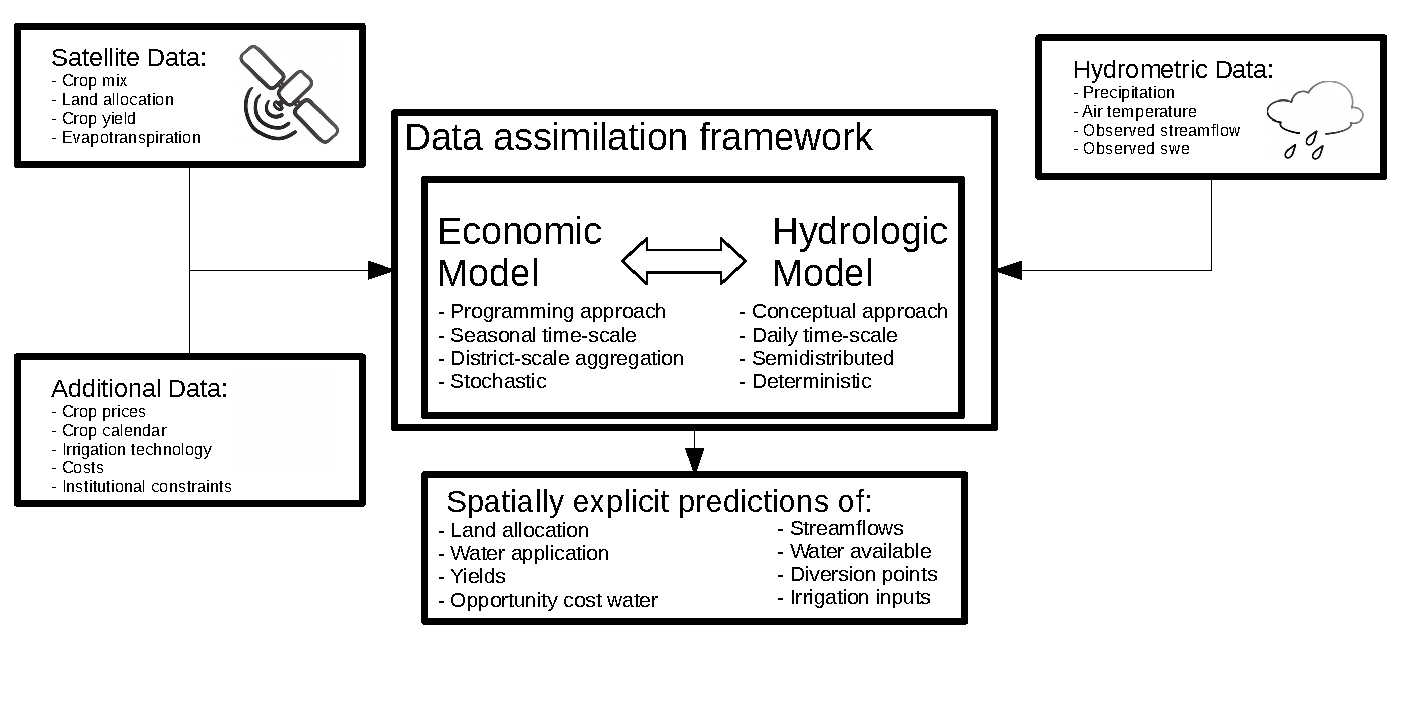
\includegraphics[width=\textwidth]{Figures/DA_approach.pdf}
    \caption{Overview of the hydro-economic modeling package. An economic model of agricultural production is linked to a spatially explicit hydrologic model and embedded in a stochastic data assimilation framework. The data assimilation framework adjusts the economic component parameters based on the ingestion of remote sensing observations of agricultural activity and other hydrometric and ancillary data. Once the model is calibrated, it can be used to predict probabilities of resource allocation under designed climate and policy scenarios.}
    \label{fig:DAFramework}
\end{figure}

\subsection{Economic model of agriculture and farmer behavior}

The backbone of the economic component is a nonlinear constrained optimization model calibrated to capture observed producer behavior using the PMP method \citep{Howitt1995}. The PMP approach is grounded in the assumption that producers allocate resources, in our case land and water, to maximize their net revenues subject to resource constraints:

% \begin{equation}\label{eq:net_revs}
%     \begin{split}
%         \max_{ x_{land,i} , x_{water,i} \geq 0 } net = \quad \sum_i \left{ p_i \pi_i\left( x_{land,i}, x_{water,1}; \mu, \beta_{land,i},\beta_{water,i}, \rho_{i}, \delta_{i} \right) \\- \left( c_{land,i} + \lambda_{land,i} \right) x_{land,i} - \left( c_{water,i} + \lambda_{water,i} \right) x_{water,i} \right} \\
%     \text{subject to} \quad\sum_{i} x_{ i 1 } \leq \overline{L} \left[ \overline{ \lambda }_{ 1 } \right]
%     \end{split}
% \end{equation}

% \begin{multline}\label{eq:net_revs}
%         \max_{ x_{land,i} , x_{water,i} } net = \quad \sum_i \left\{ p_i \pi_i\left( x_{land,i}, x_{water,i}; \mu_i, \beta_{land,i},\beta_{water,i}, \rho_{i}, \delta_{i} \right) -  c_{land,i} x_{land,i} - c_{water,i} x_{water,i} \right\} \\
%     \text{subject to: }\\ \quad\sum_{i} x_{land,i} \leq \overline{L} \left[ \overline{ \lambda }_{fsl} \right]\\
%     x_{land,i} = x_{land,i}^{obs} \left[ { \lambda }_{land,i} \right]\\
%     x_{water,i} = x_{water,i}^{obs} \left[ { \lambda }_{water,i} \right]\\
%     x_{land,i} , x_{water,i} \geq 0\\
% \end{multline}
\begin{multline}\label{eq:net_revs}
        \max_{ x_{land,i} , x_{water,i} } net = \quad \sum_i \left\{ p_i \pi_i\left( x_{land,i}, x_{water,i}; \mu_i, \beta_{land,i},\beta_{water,i}, \rho_{i}, \delta_{i} \right) -  c_{land,i} x_{land,i} - c_{water,i} x_{water,i} \right\} \\
    \text{subject to: }\\ 
    \quad\sum_{i} x_{land,i} \leq \overline{L} \left[ \overline{ \lambda }_{L} \right]\\
    \quad\sum_{i} x_{water,i} \leq \overline{W} \left[ \overline{ \lambda }_{W} \right]\\
    x_{land,i} , x_{water,i} \geq 0\\
\end{multline}

\noindent where $net$ is net revenue, defined as revenue less the costs of land and water use; the index $i = 1,...,I$ represents crops; $x_{land,i}, x_{water,i}$ represent land and water resource inputs for crop $i$, respectively; $p_i$ is the price received for crop $i$; $\pi_i$ is a production function that maps resource inputs to total production of crop $i$; and $c_{land,i}$, $c_{water,i}$ are the unit costs associated with land and water use to produce crop $i$. The parameters $\mu, \beta, \rho, \delta$ are production function parameters to be calibrated using PMP. The constraints in problem (1) state that the total land and water used for all crops in the region must be less than or equal to the total land $\overline{L}$ and water $\overline{W}$ available for cultivation and that resource allocation has to be non-negative. The total land and water available for cultivation may be constrained by physical limits (e.g., streamflow) or by policy or other institutional constraints (e.g., water rights or storage release policies). 

Consistent with the recent economic literature on PMP \citep{Merel2011b}, we define the production function in Eq. \eqref{eq:net_revs} using a generalized constant elasticity of substitution (CES) functional form: 

\begin{align}\label{eq:produc_func}
    \pi_i = \mu_i \left[ \beta_{land,i} x_{land,i} ^ { \rho_i } + \beta_{water,i} (x_{water,i} + x_{precip,i}) ^ {\rho _i} \right]^{ \frac { \delta_i}{ \rho_i} }
\end{align}

A limitation of previous research in this area is that it has differentiated the production function in Eq. \eqref{eq:produc_func} for irrigated and non-irrigated crops, requiring independent calibration of each function \citep[e.g.][]{Maneta2009c}. In this study, we streamline calibration by incorporating a production function that can handle irrigated and non-irrigated cases. To do so, we separate the total amount of water available to support crop growth into an exogenous component provided by natural sources like precipitation $x_{precip,i}$ (not controlled by the farmer), and an endogenous component provided by supplemental irrigation, $x_{water,i}$ (controlled by the farmer). This formulation also allows us to differentiate the costs of providing water for crop production, which differ depending on whether a year has relatively wet or dry conditions. %Therefore, equation \eqref{eq:net_revs} defines $x _ { i 2 } ^ { * } = x _ { 20 } + x _ { i 2 }$, where $x_{20}$ is natural ET and $x_{i2}$ is applied ET (irrigation).

\subsection{Hydrologic component}

The hydrologic component provides water availability constraints to agricultural production. Precipitation is transformed into runoff using a gridded version of the HBV model \citep{Bergstrom1973, Bergstrom1995, Lindstrom1997}. When runoff reaches the channel it is routed through the stream network using the Muskingum-Cunge method \cite{Cunge1969}. Both models are well-known and documented, and because of its parsimonious nature, reliability, robustness, and performance they have been widely applied in many regions of the world for hydrologic response analysis under climate change and drought \citep{Driessen2010, Menzel2002}. 

HBV is a precipitation-runoff model originally developed to assist in flood forecasting in Sweden. The hydrologic system is conceptualized as a cascade of four compartments: snowpack, soil, upper groundwater zone, and lower groundwater zone in each of the hydrologic response units (HRUs) in which the user may divide the region (Appendix \ref{app:hydrologic_model}). Water outputs from the soil and groundwater compartments of each HRU are transformed into runoff by convolution with a triangular unit hydrograph. We implemented this particular application as a partially gridded version of the original model. The model uses gridded (raster) daily precipitation, and maximum and minimum daily air temperature and produces the aggregated (spatially averaged) runoff response of the different subcatchments composing the study area. Water ponded on the surface of pixel $k$ at time $t$ available for infiltration and for the generation of runoff is the integration of water input rates from snowmelt $Melt_{k,t}$, rainfall $Rain_{k,t}$  and supplemental irrigation $P^{irr}_{k(j),t}$ if pixel $k$ is in the set of pixels designated to be irrigated from water source $j$,

\begin{align}
Pond_{k,t} &= Pond_{k,t-1} + (Melt_{k,t} + Rain_{k,t} +  P^{irr}_{k(j),t})\Delta t - \Delta SM_{k,t} 
\end{align} 

Infiltration (described in \ref{app:hydrologic_model}) increases the water storage in the soil ($\Delta SM_{k,t}$) at pixel $k$ and is aggregated over all pixels $k$ within subcatchment $l$. When water stored in the soil moisture compartment of subcatchment $l$ reaches a threshold, the excess water generates output or percolates to the groundwater compartment. Outputs from the soil and groundwater compartments produce the integrated response of the subcatchment. A comprehensive description of our particular implementation of the model is provided in \ref{app:hydrologic_model}. In total, the hydrologic model tracks four internal states in each of the subcatchments: snow water equivalent, soil water storage, water storage in the upper groundwater compartment and water storage in the deep water compartment. The model has \num{12} parameters that can be potentially tuned. Details of the model structure and implementation are provided in \ref{app:hydrologic_model}. 

The runoff response of each subcatchment becomes lateral water contributions into the stream reach contained in the subcatchment. Lateral runoff and inflows from upstream subcatchments are routed through the river network using the Muskingum-Cunge model. The Muskingum model uses a two-parameter constitutive equation to relate storage ($S$) in a reach to its inflows ($Q_{in}$) and outflows ($Q_{in}$): $S = K\left[eQ_{in} + (1 - e)Q_{out}\right]$, where $K$ and $e$ are the two function parameters.  This constitutive relationship permits to write the mass balance equation for the reach as a function of streamflows and parameters. The Muskingum-Cunge method uses this relationship to develop a finite difference approximation of the 1D diffusion equation:

\begin{align}
&Q_j^{t+1}\left[K_j(1 - e_j) + 0.5\Delta t  \right] + Q_{j-1}^{t+1}\left[K_je_j - 0.5\Delta t  \right]  \\
&= Q_j^{t}\left[K_j(1 - e_j) - 0.5\Delta t  \right] + Q_{j-1}^{t}\left[K_je_j + 0.5\Delta t  \right]\\
&+ (q_{j}^{t+1} - q^{irr}_{j,i,t+1}) \left[K_j(1 - e_j) + 0.5\Delta t  \right]
\end{align}

Full details on the Muskingum-Cunge algorithm and its implementation  are provided in \ref{app:hydrologic_model}.


\subsection{Model coupling}

The hydrologic component of the model operates deterministically at daily time steps and at variable spatial resolutions defined by the size of the HRUs. On the other hand, the economic component operates stochastically at seasonal time steps and at spatial resolutions defined by counties, districts, or regions that may or may not be coincident with the HRUs. To couple the two components, relevant information generated by one component needs to be spatially and temporally aggregated or disaggregated to match the resolution of the receiving component. At the beginning of each simulated year, the economic component is run over each economic unit in the domain and the probabilistic ensemble of land $\mathbf{x}_{land, i}$ and water $\mathbf{x}_{water, i}$ allocated to each crop $i$ for the growing season are determined. The average of the ensemble of seasonal water allocations $\mathbb{E}[\mathbf{x}_{water, i}]$ are temporally disaggregated to obtain expected daily diversions from the hydrologic network. Diverted water is then allocated to irrigated fields as supplemental precipitation. The temporal disaggregation of the seasonal irrigation volume to daily water diversion rates is achieved by redistributing the total crop water requirements over the growing season according to the growth stage of the crop as reflected by its crop coefficient:    

\begin{align}
    &q^{irr}_{j,i,t+1} = \frac{  \mathbb{E}[\mathbf{x}_{water, i}]*\omega_{t}}{I_{eff_i}}\\
     \nonumber &\text{where: }\\ 
    &\omega_{i,t+1} = \frac{Kc_{i,t+1}}{\sum_t Kc_{i,t+1}},
\end{align}

\noindent where $q^{irr}_{j,i,t+1}$ is the water diverted for irrigation from river node $j$ for crop $i$ at day $t+1$, $I_{eff_i}$ is an irrigation and conveyance efficiency factor for crop $i$, and $\omega_{i,t+1}$ is a weight factor that reflects the daily fraction of the total crop water requirement according to the crop coefficient $Kc_{i,t+1}$.

Water diverted each day from a given river node is applied as supplemental irrigation over pixels with land use designated as irrigated crop in the corresponding economic unit. Irrigation is applied uniformly over all pixels designed as irrigated crops: 

\begin{align}
    P^{irr}_{k(j),t+1} = \frac{\sum_i q^{irr}_{j,i,t+1} }{N_k, \Delta x^2},
\end{align}

\noindent where $P^{irr}_{k(j),t}$ is the supplemental irrigation applied at time $t$ on pixel $k$ from the set of pixels classified as irrigated agriculture within the economic unit associated with diversion point $j$, $N_k$ is the total number of pixels classified as irrigated agriculture within the economic units, and $\Delta x^2$ is the pixel area. 
 

\section{Calibration of the economic component}

\subsection{Positive Mathematical Programming}

The PMP approach assumes that farmers allocate limited land and water resources with the objective of maximizing net revenues, and thus past observations of land and water use by crop ($\overline{x}_{land,i}, \overline{x}_{water,i}$) are solutions to the problem in Eq. \eqref{eq:net_revs}. During calibration, Eq. \eqref{eq:net_revs} is modified to constrain the maximization problem to the observed levels of land and water allocation:

\begin{multline}\label{eq:net_revs_calib}
        \max_{ x_{land,i} , x_{water,i} } net = \quad \sum_i \left\{ p_i \pi_i\left( x_{land,i}, x_{water,i}; \mu_i, \beta_{land,i},\beta_{water,i}, \rho_{i}, \delta_{i} \right) -  c_{land,i} x_{land,i} - c_{water,i} x_{water,i} \right\} \\
    \text{subject to: }\\ \quad\sum_{i} x_{land,i} \leq \overline{L} \left[ \overline{ \lambda }_{fsl} \right]\\
    x_{land,i} = \overline{x}_{land,i} \left[ { \lambda }_{land,i} \right]\\
    x_{water,i} = \overline{x}_{water,i} \left[ { \lambda }_{water,i} \right]\\
    x_{land,i} , x_{water,i} \geq 0\\
\end{multline}


Equation \eqref{eq:net_revs_calib} contains seven parameters per crop: five production function parameters  $\mu_i, \beta_{i,land}, \beta_{i,water}, \rho_i, \delta_i$, and two Lagrange multipliers associated with the observed land and water-use constraints $\lambda_{i, land}, \lambda_{i,water}$, for a total of 7 unknown parameters to be calibrated based on observed decision making. An additional parameter, $\overline{\lambda_{fsl}}$ associated with the land resource constraint also needs to be calibrated. This parameter represents the shadow value for the total amount of land available for crop production.  %Parameter $\overline{\lambda_{fsl}}$, $\lambda_{land,i}$ and $\lambda_{water,i}$ are Lagrange multipliers associated with the resource constraints. 
The PMP methodology builds the system of optimality conditions associated with Eq. \eqref{eq:net_revs_calib}, however instead of solving the maximization problem to find optimal land and water resource allocation, the method fixes these at the observed allocation levels and solves the system of optimality conditions for the model parameters. In essence, the PMP methodology finds the parameters that produce a response surface (net revenue function) that is maximum at the observed resource allocation levels ($\overline{x}_{land,i}, \overline{x}_{water,i}$). Eq. \ref{eq:net_revs_calib} is differentiable and traditionally solved using nonlinear programming methods. Necessary and sufficient optimality conditions are given by the first order derivatives of Eq. \ref{eq:net_revs_calib} with respect to $x_{land,i}$ and $x_{water,i}$, the Karush-Kuhn-Tucker conditions to enforce constraints, and a few additional constraints to ensure the solution to the maximization problem exists and is unique.  A programming solution to Eq. \ref{eq:net_revs_calib}, proposed by Merel et al. \citet{Merel2011b} and used in this study, is provided in \ref{app:economic_model_calib}.  



\subsection{Stochastic Recursive Parameter Estimation}

Instead of solving the program proposed by Merel et al. \citet{Merel2011b} and Garnache et al. \citep{Garnache2017}, we embed the optimality conditions within a stochastic data assimilation framework that permits the recursive calibration of the model parameters. \citet{Maneta2014} describe a discrete Monte Carlo recursive Bayesian estimator that permits to update the parameters as new observations become available at time $k$. The proposed methodology has three important advantages: 1) its probabilistic nature permits to include noisy observations (e.g. remotely sensed retrievals of agricultural activity) in the parameter estimation process; 2) it provides a posterior parameter distribution that integrates old and new information; and 3) it does not require the history of observations to update the calibration when new observations are obtained. 

The equations of the estimator are based on the ensemble Kalman Filter, enKF \citep{Evensen1994}, where the probability distribution of parameters, inputs and observations are represented by a Monte Carlo sample. The exception is parameter $\rho_i$, a function of $\sigma_i$, which controls the elasticity of substitution between land and water. This parameter is fixed at a value $\rho_i = \frac{\sigma_i - 1}{\sigma_i}$, with $\sigma_i$ values typically in the range of 0.1 to 0.6, which represents limited substitution between these two resources. The reason for fixing this parameter is that elasticity of substitution has been found to be insensitive to aggregated observations and requires more detailed experimental data for its identification. Therefore, our approach stochastically tracks seven parameters, six parameters that need to be calibrated for each crop, and one unit-level resource constraint parameter ($\overline{\lambda}_{fsl}$). Specifically, the probability distribution of the model parameters $\*\theta = \{\*\mu,\allowbreak \*\beta_{land},\allowbreak \*\beta_{water}, \*\delta,\allowbreak \*\lambda_{land},\allowbreak \*\lambda_{water},\allowbreak \overline{\lambda}_{fsl}\}$ is represented by a random ensemble of $M$ members $m=1,...,M$ of $\*\theta$. Except for $\overline{\lambda}_{fsl}$, the unit-level parameter, each bold parameter in the $\*\theta$ set is an array with rows representing parameter values for each crop grown in a given economic unit (e.g. county, irrigation district) and each column is an individual member of the ensemble.

To set the filter equations, we treat model parameters as if they were the system states of the standard enKF. The evolution of parameters (forecasts) from period $k$ to $k+1$ is produced by adding a random perturbation to each member of the ensemble. The addition of artificial noise to each ensemble member to simulate time dynamics results in an overdispersed ensemble that overestimates the parameter variance \citep{West1993}. This is because the intrinsic variance of the ensemble is compounded by the noise added to each member to perform the random walk. Liu and West \citep{West1993} show that this can be corrected by using perturbations that are proportional to the ensemble variance by a number $h$ slightly smaller than one, and shrinking the ensemble toward its mean by a factor $a = \sqrt{1-h}$. For a given crop $i$,  the dynamics of members of the parameter ensemble with shrinkage is:   

% \begin{equation}\label{eq:param_evolution}
%     \underbrace{\begin{bmatrix}
%     \*\mu_{k+1}^{m}\\ 
%     \*\beta_{land,k+1}^{m}\\ 
%     \*\beta_{water,k+1}^{m}\\ 
%     \*\delta_{k+1}^{m}\\ 
%     \*\lambda_{land,k+1}^{m}\\ 
%     \*\lambda_{water,k+1}^{m}\\ 
%     \overline{\lambda}_{fsl,k+1}^{m}\\
%     \end{bmatrix}}_{\*\theta_{k+1}^m} = a
%     \begin{bmatrix}
%     \*\mu_k^{m+}\\ 
%     0\\ 
%     0\\ 
%     \*\delta_k^{m+}\\ 
%     \*\lambda_{land,k}^{m+}\\ 
%     \*\lambda_{water,k}^{m+}\\ 
%     \overline{\lambda}_{fsl,k}^{m+}\\
%     \end{bmatrix} + (1 - a)
%     \begin{bmatrix}
%     \mathbb{E}[\*\mu_{k}^+]\\ 
%     0\\
%     0\\ 
%     \mathbb{E}[\*\delta_k^{+}]\\ 
%     \mathbb{E}[\*\lambda_{land,k}^{+}]\\ 
%     \mathbb{E}[\*\lambda_{water,k}^{+}]\\ 
%     \mathbb{E}[\overline{\lambda}_{fsl,k}^{+}]\\
%     \end{bmatrix} +
%     \begin{bmatrix*}[l]
%     \*\zeta_{k}^\mu\\ 
%     \*\zeta_{k}^{\beta_{land}}\\
%     \*\zeta_{k}^{\beta_{water}}\\
%     \*\zeta_{k}^\delta\\
%     \*\zeta_{k}^{\lambda_{land}}\\
%     \*\zeta_{k}^{\lambda_{water}}\\
%     \*\zeta_{k}^{\overline{\lambda}_{fsl}}
%     \end{bmatrix*}\text{,} \qquad 
%     \begin{matrix*}[l]
%     &\*\zeta_k^\mu \sim \mathcal{N}\left(0, h^2\*Z_k^{\*\mu} \right)\\
%     &\*\zeta_{k}^{\beta_{land}} \sim \mathcal{B}\left(\hat{\*a}(\*\beta_{land,k}^{+}), \hat{\*b}(\*\beta_{land,k}^{+}) \right)\\
%     &\*\zeta_{k}^{\beta_{water}} \sim \mathcal{B}\left(\hat{\*a}(\*\beta_{water,k}^{+}), \hat{\*b}(\*\beta_{water,k}^{+}) \right)\\
%     &\*\zeta_{k}^\delta \sim \mathcal{N}\left(0, h^2\*Z_{k}^{\*\delta} \right)\\
%     &\*\zeta_{k}^{\lambda_{land}} \sim \mathcal{N}\left(0, h^2\*Z_{k}^{\*\lambda_{land}} \right)\\
%     &\*\zeta_{k}^{\lambda_{water}} \sim \mathcal{N}\left(0, h^2\*Z_{k}^{\*\lambda_{water}} \right)\\
%     &\*\zeta_{k}^{\overline{\lambda}_{fsl}} \sim \mathcal{N}\left(0, h^2\*Z_{k}^{\overline{\lambda}_{fsl}} \right)
%     \end{matrix*}
% \end{equation}

\begin{equation}\label{eq:param_evolution}
    \underbrace{\begin{bmatrix}
    \beta_{land,i,k+1}^{m}\\ 
    \beta_{water,i,k+1}^{m}\\
    \mu_{i,k+1}^{m}\\ 
    \delta_{i,k+1}^{m}\\ 
    \lambda_{land,i,k+1}^{m}\\ 
    \lambda_{water,i,k+1}^{m}\\ 
    \overline{\lambda}_{fsl,k+1}^{m}\\
    \end{bmatrix}}_{\*\theta_{i,k+1}^m} = a
    \begin{bmatrix}
    0\\ 
    0\\
    \mu_{i,k}^{m+}\\ 
    \delta_{i,k}^{m+}\\ 
    \lambda_{land,i,k}^{m+}\\ 
    \lambda_{water,i,k}^{m+}\\ 
    \overline{\lambda}_{fsl,k}^{m+}\\
    \end{bmatrix} + (1 - a)
    \begin{bmatrix}
    0\\
    0\\
    \mathbb{E}[\*\mu_{i,k}^+]\\ 
    \mathbb{E}[\*\delta_{i,k}^{+}]\\ 
    \mathbb{E}[\*\lambda_{land,i,k}^{+}]\\ 
    \mathbb{E}[\*\lambda_{water,i,k}^{+}]\\ 
    \mathbb{E}[\overline{\*\lambda}_{fsl,k}^{+}]\\
    \end{bmatrix} +
    \begin{bmatrix*}[l]
    \zeta_{i,k}^{\beta_{land}}\\
    \zeta_{i,k}^{\beta_{water}}\\
    \zeta_{i,k}^\mu\\ 
    \zeta_{i,k}^\delta\\
    \zeta_{i,k}^{\lambda_{land}}\\
    \zeta_{i,k}^{\lambda_{water}}\\
    \zeta_{k}^{\overline{\lambda}_{fsl}}
    \end{bmatrix*}\text{,} \qquad 
    \begin{matrix*}[l]
    &\zeta_{i,k}^{\beta_{land}} \sim \mathcal{B}\left(\hat{a}_i(\*\beta_{land,k}^{+}), \hat{b}_i(\*\beta_{land,k}^{+}) \right)\\
    &\zeta_{i,k}^{\beta_{water}} \sim \mathcal{B}\left(\hat{a}_i(\*\beta_{water,k}^{+}), \hat{b}_i\*\beta_{water,k}^{+}) \right)\\
    &\zeta_{i,k}^\mu \sim \mathcal{N}\left(0, h^2\mathbb{V}[\mu_{i,k}^+] \right)\\
    &\zeta_{i,k}^\delta \sim \mathcal{N}\left(0, h^2\mathbb{V}[\delta_{i,k}^+] \right)\\
    &\zeta_{i,k}^{\lambda_{land}} \sim \mathcal{N}\left(0, h^2\mathbb{V}[\lambda_{land,i,k}^+] \right)\\
    &\zeta_{i,k}^{\lambda_{water}} \sim \mathcal{N}\left(0, h^2\mathbb{V}[\lambda_{water,i,k}^+] \right)\\
    &\zeta_{k}^{\overline{\lambda}_{fsl}} \sim \mathcal{N}\left(0, h^2\mathbb{V}[\overline{\lambda}_{fsl,k}^+] \right)
    \end{matrix*},
\end{equation}

\noindent where superscript $m$ over a a parameter indicates it is the $m$th ensemble member at the time indicated by the subscript $k$, and superscript $+$ indicates the parameter is corrected (posterior) after data assimilation at time $k$ (see below); $a$ and $h$ are shrinkage and variance smoothing parameters, respectively; $\mathbb{E}[\cdot]$ is the expectation operator of the parameter ensemble (i.e. ensemble average for the given parameter and crop), and operator $\mathbb{V}[\cdot]$ is the parameter ensemble variance. Parameters $\mu, \delta, \lambda_{land}, \lambda_{water} \text{ and } \overline{\lambda}_{fsl}$ are sampled using normally distributed noise, however the $\beta$ parameters are bound to values in the range [0,1]. To sample the distribution of these parameters at $k+1$ we used a Beta distribution with two shape parameters, $\hat{a}, \hat{b}$ centered at each ensemble member. The parameters that center the distribution at each member are determined using the method of moments from the mean and the variance of each individual ensemble member: 

% \begin{equation}\label{eq:beta_params}
%     \begin{split}
%     &\hat{\*a}(\*\beta) = \left[\hat{a}_i(\*\beta), \dots, \hat{a}_I(\*\beta) \right]^T, \qquad \hat{a}_i(\*\beta) = \overline{\*\beta}_i^m\left(\frac{\overline{\*\beta}_i^m(1-\overline{\*\beta}_i^m)}{\*Z^{\*\beta}_{ii}} -1 \right)\\
%     &\hat{\*b}(\*\beta) = \left[\hat{b}_i(\*\beta), \dots, \hat{b}_I(\*\beta) \right]^T, \qquad \hat{b}_i(\*\beta) = (1-\overline{\beta}_i^m)\hat{a}_i(\beta_i),
%     \end{split}
% \end{equation}
\begin{equation}\label{eq:beta_params}
    \begin{split}
    &\hat{a}_i(\beta_{\cdot}) = <\*\beta_{\cdot,i}^m>\left(\frac{<\*\beta_{\cdot,i}^m>(1-<\*\beta_{\cdot,i}^m>)}{\mathbb{V}[\beta_{\cdot,i,k}^+]} -1 \right)\\
    &\hat{b}_i(\*\beta_{\cdot}) = (1-<\*\beta_{\cdot,i}^m>)\hat{a}_i(\beta_{\cdot,i}),
    \end{split}
\end{equation}
 \noindent where $<\*\beta_{\cdot,i}^m>$ is the mean of the kernel locations and $Var(\*\beta^m)$ is the variance of the ensemble:
\begin{equation}
\begin{split}
    &<\*\beta_{\cdot,i}^m> = a\*\beta_{\cdot,i,k}^{m+} + (1-a)\mathbb{E}[\*\beta_{\cdot,i,k}^{+}] \\
\end{split}
\end{equation}

Uncertainty in remote sensing observations of agricultural activity (land and water allocations, crop yield and yield elasticity) as well as uncertainty in additional ancillary information (crop supply elasticity, crop price, cost of operating land and cost of water) obtained at time $k+1$ is represented by generating an ensemble with $M$ observations of replicates obtained by sampling from a Normal distribution centered at the observation:

\begin{equation}
    \begin{split}
        &\overline{x}_{land,i,k+1}^m = \overline{x}_{land,i} + \nu_{land,i,k+1}^m, \qquad  \nu_{land,i,k+1}^m \sim \mathcal{N}\left(0, R_{k+1}^{x_{land}} \right)\\
        &\overline{x}_{water,i,k+1}^m = \overline{x}_{water,i} + \nu_{water,i,k+1}^m, \qquad  \nu_{water,i,k+1}^m \sim \mathcal{N}\left(0, R_{k+1}^{x_{water}} \right)\\
        &\overline{\pi}_{W,i,k+1}^m = \overline{\pi}_{W,i,k+1} + \nu_{\pi_W,i,k+1}^m, \qquad  \nu_{\pi_W,i,k+1}^m \sim \mathcal{N}\left(0, R_{k+1}^{\pi_W} \right)\\
        &\overline{\pi}_{i,k+1}^m = \overline{\pi}_{i,k+1} + \nu_{\pi,i,k+1}^m, \qquad  \nu_{\pi,i,k+1}^m \sim \mathcal{N}\left(0, R_{k+1}^{\pi} \right)\\
        &\overline{\eta}_{i,k+1}^m = \overline{\eta}_{i,k+1} + \nu_{\eta,i,k+1}^m, \qquad  \nu_{\eta,i,k+1}^m \sim \mathcal{N}\left(0, R_{k+1}^{\eta} \right)\\
        &p_{i,k+1}^m = p_{i,k+1} + \nu_{p,i,k+1}^m, \qquad  \nu_{p,i,k+1}^m \sim \mathcal{N}\left(0, R_{k+1}^{p} \right)\\
        &c_{land,i,k+1}^m = c_{land,i} + \nu_{cland,i,k+1}^m, \qquad  \nu_{cland,i,k+1}^m \sim \mathcal{N}\left(0, R_{k+1}^{c_{land}} \right)\\
        &c_{water,i,k+1}^m = c_{water,i} + \nu_{cwater,i,k+1}^m, \qquad  \nu_{cwater,i,k+1}^m \sim \mathcal{N}\left(0, R_{k+1}^{c_{water}} \right),
    \end{split}
\end{equation}

\noindent where $\overline{x}_{land,i}^m, \overline{x}_{water,i}^m, \overline{\pi}_{W,i}, \overline{\pi}_{W,i}, \text{ and } \overline{\eta}_i $, are observations of land and water used by crops, elasticity of production to water inputs, crop production, and elasticity of production to crop prices, respectively. Observations are scaled into a dimensionless quantity (see section \ref{sec:scaling_obs}). 
    
Assimilation of new observations obtained at time $k+1$ to correct each member $m$ of the parameter ensemble is achieved using the update equations of the enKF:  

\begin{equation}\label{eq:recursive_bayes}
    \begin{split}
    &\theta_{i,k+1}^{m+} = \theta_{i,k+1}^{m} + K_{k+1} \left( LHS^m_{i,k+1} - RHS(\theta_{i,k+1}^{m})\right)\\
    &K_{k+1} = \*C^{\theta,RHS}_{k+1} \left[\*C^{LHS}_{k+1} + \*C^{RHS}_{k+1}\right]^{-1},\\
    \end{split}
\end{equation}

\noindent where $\theta_{i,k+1}^{m+}$ is the corrected (posterior) $m$th member of the model parameters, $K_{k+1}$ is the Kalman gain matrix that corrects the parameter trajectories; ${LHS}^m_{i,k+1}$ is the $m$th member of the ensemble of replicates of the left hand side of the system of optimality conditions, which holds observation and other derived quantities; $RHS(\theta_{i,k+1}^{m})$ is the $m$th member of the ensemble of replicates of the right hand side of the optimality conditions, which is a function of model parameters, and holds predictions of the $LHS$;   $\*C^{\theta,LHS}_{k+1}$  is the cross-covariance between the parameter ensemble and the RHS ensemble, $\*C^{LHS}_{k+1}$ is the covariance of the LHS ensemble and $\*C^{RHS}_{k+1}$ is the covariance of the RHS ensemble. 

The quantity between brackets in the top equation of \eqref{eq:recursive_bayes} is called the innovation and holds the model prediction errors. A property of Kalman filters is that when they are properly tuned, the ensemble of parameters produce a sequence of innovations that is normally distributed with zero mean. Since LHS and RHS represent the left and right hand sides of the optimality conditions, Eq. \ref{eq:recursive_bayes} is in effect solving the maximization problem posed in Eq. \ref{eq:net_revs}. The variance of the innovation is the total variance of the process associated with observation and parameter uncertainty. 


% Symbols in boldface within $\*\theta$ indicate vectors of parameters for all crops in an economic unit(i.e $\*\mu = [\mu_1,\dots, \mu_I]^T$).  

% where $\*\theta_{k+1}^m$ is an augmented vector concatenating vectors of parameters that hold individual parameter values for each crop grown in a given economic unit:

% \noindent where $\*K_k$ is the Kalman gain, $\*{LHS}_k$ is the left hand side of the optimality conditions (left hand side of \eqref{eq:optimality_program}), which represent the marginal costs of agricultural production and other observations of agricultural activity:

% \begin{equation}
% \*{LHS}^m = \left[ LHS_i^m,\dots,LHS_I^m\right]^T,
% \end{equation}

The $LHS_i$ ensemble is produced by reorganizing the nonlinear system of optimality conditions (Eq.\eqref{eq:optimality_program}) such that observed quantities are grouped in the left hand side of the system. Using the observation replicates, individual $LHS_i$ ensemble members are produced:

\begin{equation}
LHS_{i, k+1}^m = 
\begin{blockarray}{ccc}
\begin{block}{[c]cc}\label{eq:LHS}
    -p_i^m\, \overline{\pi}_i^m \, \overline{\pi}_{W,i}^m & &(1)\\
    p_i^m \,\overline{\pi}_i^m \, \overline{\pi}_{W,i}^m & &(2)\\
    \overline{\eta_i}^m & &(3)\\
    \overline{\pi}_{W,i}^m& &(4)\\
    \overline{\pi_i}^m& &(5)\\
    \sum_{i=0}^{I} \left(2\, \overline{x}_{land,i}^m \,p_i^m \,\overline{\pi}_i^m \,\overline{\pi}_{W,i}^m \right) & &(6)\\
    1& &(7)\\
    0& &(8)\\
    0&_{k+1} &(9)\\ 
\end{block}
\end{blockarray}
\end{equation}

\noindent where the first two elements are part of the calculation of the marginal costs of production, the next two elements are observations of production elasticity to crop price and used water, respectively, the fifth element is the observations of crop production and the last three elements are the left hand side of three constraints to encourage sampling $\beta$ parameters such as $\beta_{land,i} + \beta_{water,i}=1, \beta_{\cdot,i}\geq 0$.

The $RHS(\theta_{k+1})$ ensemble is the right hand side of the optimality conditions, which is a function of model parameters. Using parameter and input replicates, the right hand side equations are used to produce model prediction replicates of $LHS_{i, k+1}$:

% \begin{equation}\label{eq:RHS}
%     \*{RHS}(\*\theta_k^{m}) = \left[ RHS(\*\theta_{i,k}^{m}),\dots,RHS(\*\theta_{I,k}^{m})\right]^T,
% \end{equation}

\begin{equation}
    RHS(\theta_{i,k+1}^{m}) = 
    \begin{blockarray}{cccc}
    \begin{block}{[cc]cc}\label{eq:RHS}
        & \left(c_{land,i}^m + \lambda_{land,i}^m + \overline{\lambda}_{fsl}^m \right) \overline{x}_{land,i}^m - p_i^m\, \overline{\pi}_i^m \,\delta_i^m & &(1)\\
        & \left(c_{water,i}^m + \lambda_{water,i}^m \right) \overline{x}_{water,i}^{*m} & &(2)\\
        & \frac{\delta_i^m} {1 - \delta_i^m} \left\{1 - \frac{\frac{b_i} {\delta_i^m \left(1 - \delta_i^m\right)}}{\sum_{i}\left[\frac{b_{i}}{\delta_i^m\left(1-\delta_i^m \right) } + \frac{\sigma_{i}^m b_i\overline{\pi}_{W,i}^m} {\delta_i^m\left(\delta_i^m - \overline{\pi}_{W,i}^m \right) }\right]}\right\}, \quad b_{i} = \frac{(\overline{x}_{land,i}^{m})^2}{p_{i}^m\,\overline{\pi}_{i}^m}  & &(3)\\
        & \delta_{i}^m\left(\frac{\beta_{water,i}^m(\overline{x}_{water,i }^m)^{*\rho_i}} {\beta_{land,i }^m(\overline{x}_{land,i}^m)^{\rho_i} + \beta_{water,i}^m (\overline{x}_{water,i}^m)^{*\rho_i}} \right) & &(4)\\
        & \mu_i^m \left[\beta_{land,i}^m(\overline{x}_{land,i}^m)^{\rho_i} + \beta_{water,i}^m(\overline{x}_{water,i}^m)^{*\rho_i} \right]^{\frac{\delta_i^m}{\rho_i}} & &(5)\\
        & \sum_{i=0}^I \left[ -2 (c_{land,i}^m + \overline{\lambda}_{fsl}^m)\, (\overline{x}_{land,i}^m)^2 + 2\,\overline{x}_{land,i}^m\,p_i^m\,\overline{\pi}_i^m\,\delta_i^m \right] & &(6)\\
        & \beta_{land_i}^m + \beta_{water_i}^m & &(7)\\
        & \beta_{land_i}^m - \lvert \beta_{land_i}^m \rvert & &(8)\\
        & \beta_{water_i}^m - \lvert \beta_{water_i}^m \rvert &_{k+1} &(9)\\
\end{block}
\end{blockarray}
\end{equation}

The first two elements of $LHS_i^m$ and $RHS_i^m$ represent the difference between marginal costs of production and marginal revenues with respect to land and water. Marginal costs and marginal revenues are equal at the optimal point. The next two elements of $RHS_{i,k+1}^m$ are model predictions of production elasticity to crop price and used water, respectively; the fifth element is the observation of crop production. The last three elements of $LHS_i^m$ and $RHS_i^m$ are constraints to encourage sampling   $\beta$ parameters within the unit simplex, such as $1 = \beta_{land,i} + \beta_{water,i}, \beta_{\cdot,i}\geq 0$. The last two constraints are the non-negativity conditions. Non-negative $\beta$ samples occur when the difference between the sample and its absolute is zero.  


\subsection{Scaling observations and inputs}\label{sec:scaling_obs}

If the $\beta$ parameters are considered dimensionless share quantities, the constant elasticity of substitution production function specified in Eq. \eqref{eq:produc_func} is dimensionally inconsistent and its results are not interpretable in terms of processes unless inputs are scaled and transformed to dimensionless quantities. For a particular season, the information needed to correct the model parameters for an economic unit include observations of land ($x^{obs}_{land,i}$, \si{\hectare}) and water ($x^{obs}_{water,i}$ \si{\milli\meter\per\hectare}) used by crop $i$, crop price ($p^{obs}_i$, \$\si{\per\tonne}), the typical cost of cultivating crop $i$ per unit of land ($c^{obs}_{land}$ \$\si{\per\hectare}), the cost of applying a unit of water including fees, transportation, application costs, etc ($c^{obs}_{water}$ \$/(\si{\milli\meter\hectare}), average crop yield over the economic unit ($y^{obs}_i$, \si{\tonne\per\hectare}), the elasticity of production to water ($\pi_{Wi}^{obs}$, dimensionless), and the elasticity of production to crop prices ($\eta^{obs}_i$, dimensionless). 

The dimensionless observed quantities used in the data assimilation and parameter correction process are obtained by applying the following transformations:

\begin{equation}
    \begin{split}
        &\overline{x}_{land,i} = \frac{x^{obs}_{land,i}}{x^{ref}_{land,i}}\\
        &\overline{x}_{water,i} = \frac{x^{obs}_{water,i}}{ET^{ref}_i * x^{ref}_{land,i}}\\
        &\overline{x}_{precip,i} = \frac{x^{est}_{precip,i}}{ET^{ref}_i}\\
        &\overline{\pi}_i = \frac{y^{obs}_i x^{obs}_{land,i}}{y^{ref}_ix^{ref}_{land,i}}\\
        &p_i = \frac{p^{obs}_i}{p^{ref}_i}\\
        &c_{land,i} = \frac{c^{obs}_{land,i}}{p^{ref}_i y^{ref}_i}\\
        &c_{water,i} = x^{obs}_{water,i}\frac{ET^{ref}_i x^{ref}_{land,i}}{p^{ref}_i y^{ref}_i},\\
    \end{split}
\end{equation}

\noindent where $y^{obs}_i$ is the mean observed yield in the economic unit ($\si{\kilo\gram\per\hectare}$),  $x^{est}_{precip,i}$ is the estimated or expected crop water use from natural water sources (e.g. from precipitation) in $\si{\milli\meter}$, and $x^{ref}_{land,i}$ in $\si{\hectare}$, $ET^{ref}_i$ in $\si{\milli\meter}$, $p^{ref}_i$ in $\$\si{\per\kilo\gram}$ and $y^{ref}_i$ in $\si{\kilo\gram\per\hectare}$ are long term mean land, used water, price and yield observations used as reference scaling quantities for crop $i$.

Elasticity to water and prices measures how responsive their production is to used water and crop prices and is defined as a percent change in production over a percent change in used water or crop price. Defining $\pi^{obs}_i = y^{obs}_i x^{obs}_{land,i}$, elasticities can be calculated from observations as: 

\begin{equation}
    \label{eq:elast_water}
    \overline{\pi}_{W,i} = \frac{\Delta \pi_i^{obs}/ \pi^{obs}_i}{\Delta x^{obs}_{water,i}/x^{obs}_{water,i}} = \frac{d\log \pi^{obs}_i}{d\log x^{obs}_{water,i}}
\end{equation}
\begin{equation}\label{eq:elast_supply}
    \overline{\eta}_i = \frac{\Delta \pi^{obs}_i/ \pi^{obs}_i}{\Delta p^{obs}_i/p^{obs}_i} = \frac{d\log \pi^{obs}_i}{d\log p^{obs}_i}\\
\end{equation}

Elasticities are typically considered constant over a period of time and they can be obtained as the least square regression slope between the logarithm of production and the logarithm of water used or the logarithm of crop prices over the considered period. 

\subsection{Economic component at simulation time}

The posterior parameter distribution obtained after the most recent assimilation step $K$ is used in the production and cost functions of the net revenue equation \eqref{eq:net_revs}. For each member in the parameter ensemble, the maximization problem is solved, this time for land and water allocation under any simulation scenario represented by different crop prices, production costs, and land and water constraints: 

\begin{equation}\label{eq:net_revs_simul_time}
    \begin{split}
        \max_{x^m_{land, i} , x^m_{water, i} \geq 0 } net^m =\\
        &\quad \sum_{i} \left\{ p_i \pi^m_i\left( x_{land,1}, x_{water,i} + x_{precip,i}; \mu^{m+}_{i,K}, \beta^{m+}_{land,i,K},\beta^{m+}_{water,i,K}, \rho_{i}, \delta^{m+}_{i,K} \right) \right. \\
        &- \left(c_{land,i} + \lambda^{m+}_{land,i,K} + \overline{\lambda}^{m+}_{fsl,K} \right) x^m_{land,i} \\
        &- \left. \left( c_{water,i} + \lambda^{m+}_{water,i,K} \right) x^m_{water,i} \vphantom{\sum} \right\} \\
        \text{subject to} & \quad\sum_{i} x^m_{land,i} \leq \overline{L} \left[ \overline{ \lambda }^m_{ land } \right]\\
        & \quad\sum_{i} x^m_{water, i} \leq \overline{W} \left[ \overline{ \lambda }^m_{ water } \right]
    \end{split}
\end{equation}

Maximization of equation \eqref{eq:net_revs_simul_time} for each member $m$ of the parameter ensemble generates a result ensemble that represents the probability distribution of land and water allocated to each crop $i$ as well as an ensemble of the Lagrange multipliers $\overline{ \lambda }^m_{ land }$ and $\overline{ \lambda }^m_{ water }$ associated with  total land $\overline{L}$ and water $\overline{W}$ resource constraints imposed by physical availability or policy. Lagrange multipliers represent  the opportunity cost associated with not having an additional unit of land or water and therefore can be interpreted as a metric of the value of land and water. Additionally, solving equation \eqref{eq:net_revs_simul_time} also produces the probability distribution of estimated crop production, and of the probability distribution of production elasticity of supply and production elasticity of water inputs. 

\section{Application to Montana}

We demonstrate the application of the model at regional scales in the state of Montana, located in the intermountain Pacific northwest of the United States (inset of Figure \ref{fig:hydro_network}). The study region extends beyond the boundaries of the state to include the headwaters of basins that drain into the state, covering an area of 464,800 \si{\kilo\meter\squared}. The state has a longitudinal topographic and climatic gradient, from the steep and relatively wet Rocky mountain western region toward the flatter and significantly drier eastern portions of the state, which are part of the US northern great plains region. The US continental divide runs roughly north to south along the west quarter of the state. About 25\% of  Montana drains to the Pacific (Columbia and Clark Fork basins) and the rest of the state (headwaters of the Missouri basin) is part of the Atlantic basin. Annual precipitation inputs range from over 1000 \si{\milli\meter\per\year} in the mountain regions of the west and gradually decline to about 200 \si{\milli\meter\per\year} in eastern Montana. The western part of the state also shows less continentality, with relatively warmer temperatures in the winter and cooler temperatures in the summer than the eastern portion of the state. 

Other than the ecosystem, the largest water user in the state is agriculture. Agriculture is also a key industry in the state. Despite its economic importance, agriculture is poorly diversified and dominated in terms of production and planted area by alfalfa, wheat, and barley. Montana is a major producer of wheat and barley in the US and contributes to the country's food security. Irrigation is common along streams and in the western parts of the state, however rainfed production is dominant and very vulnerable to drought, especially in the drier central and eastern parts of the state. Irrigation has been growing substantially in the state in recent decades and has contributed to increasing production and reducing economic risk. Surface water is the primary source for irrigation in the west and within irrigation districts, and so far significant groundwater depletion due to agricultural extraction is only limited to a few localized watersheds (\citep[][p. 120]{MCA2017}).

\subsection{Implementation of hydrologic component}

The representation of the hydrologic system in the the study region is shown in Figure \ref{fig:hydro_network}. The figure shows the representative elementary watersheds (REWs) that compose the domain, the nodes that define their outlets, and the links (stream reaches) that connect them. We used the GTOPO30 digital elevation model (DEM) produced by the USGS at 1Km resolution to determine the regional drainage network and partition the domain into REWs using GIS procedures. We used the location of active National Water Information System streamflow gauges as the initial set of nodes to partition the landscape into REWS and then further densified the network with additional nodes until we achieved sufficient spatial detail. The densification was done by allocating nodes in pixels having contributing areas larger than a specified threshold. The minimimum contributing area for a REW was selected such that the total number and sizes of REWS was considered adequate to resolve the spatial variability of streamflows. The final domain contains over 300 REWS with typical sizes around 1400 \si{\kilo\meter\squared}. 

Each REW in the domain has one stream reach with a '\texttt{from\_node}' and '\texttt{to\_node}' attribute that identify the upstream and downstream node of the reach. This information is used to build the network topology and a node adjacency matrix that is used in the the water routing algorithm described in \ref{app:hydrologic_model}. Water diversions occur at 56 selected river nodes, one for each economic unit (county) included in the simulation.  

The model was run with daily gridded precipitation, maximum and minimum air temperatures at a 4\si{\kilo\meter} resolution, automatically retrieved as NetCDF files from the gridMET dataset \citep{Abatzoglou2013}. Temperatures are used internally by the model to calculate reference crop evapotranspiration using the Hargreaves method \citep{Hargreaves1985}.

\subsubsection{Calibration of hydrologic component}

The hydrologic model parameters were calibrated manually against streamflow observations at gauged river nodes and against snow water equivalent observations from the SNOTEL network. All parameters of the HBV rainfall-runoff model and Muskingum-Cunge routing model were adjusted and shared between REWs grouped according to their physiographical (mean elevation, mean slope, area, shape factor) and land use characteristics (fraction of the REW under forest cover and under agriculture) using a standard K-means classification method. In total we calibrated seven groups of parameters corresponding to seven groups of REWs.   

\begin{figure}[t]
    \centering
    \includegraphics[width=\textwidth]{Figures/HydroNetwork}
    \label{fig:hydro_network}
    \caption{Location of the study region and representation of the hydrologic system and streamflow network}
\end{figure}


\subsection{Implementation of economic component}

Although remote sensing can retrieve information about land and water allocation at field scales, the specification of the economic component of our model is designed to simulate the aggregated economic behavior of producers in a region, not the behavior of individual farms. The economic units considered in this implementation are aggregated at the county level. Thus, we are representing the agricultural system in Montana using 56 economic units (counties), each of them retrieving water from the stream network at one designated diversion node. Although the economic activity is represented in aggregated form, intra-county agroeconomic heterogeneity is, to some extent, implicitly captured in the distribution of model predictions for each county.

\subsubsection{Recursive calibration of the economic component}

Information necessary to update the model parameters include land allocated to each crop, total water used by each crop and total crop production. This information is available every year from remote sensing products at 30 m spatial resolution and then aggregated at county scales. In addition, information on crop prices, approximated variable unit costs of cultivating land and cost of applying water are also required (Table \ref{tab:econ_obs_sources}).

% Please add the following required packages to your document preamble:
% \usepackage{booktabs}
\begin{table}
\caption{Observations necessary to calibrate the economic component}
\centering
\label{tab:econ_obs_sources}
\begin{tabular}{@{}lllll@{}}
\toprule
Observation                    & Units      & Source         & Resolution  \\ \midrule
Land allocation                & ha         & Remote sensing \citep{USDAa} & 30 m, 8 day \\
Water allocation               & mm*ha (decastere)      & Remote Sensing \citep{He2019} & 30 m, 8 day  \\
Crop price                     & \$/ton     & USDA           & State-level, Annual  \\
Cost of land                   & \$/ha      &                & State-level, Annual  \\
Cost of water                  & \$/(mm*ha) &                & State-level, Annual  \\
Crop yield                     & ton        & Remote Sensing \citep{He2018} & 30 m, 8 day   \\
Production elasticity to water & -          & Derived, Eq \eqref{eq:elast_water}        & State-level, Annual  \\
Production elasticity to price & -          & Derived, Eq \eqref{eq:elast_supply}        & State-level, Annual \\ \bottomrule
\end{tabular}
\end{table}

Crop price information and an approximation of production costs were obtained from annual surveys published by the U.S. Department of Agriculture National Agricultural Statistics Service (USDA NASS) at the state scale (QuickStats, \url{http://quickstats.nass.usda.gov}). Crop coefficients to determine crop development stage were obtained from tables published by the AgriMet network for crops grown in the US Pacific Northwest (\url{https://www.usbr.gov/pn/agrimet/cropcurves/crop_curves.html}). 
%Include narrative about data uncertainty. 

Annual variations in crop mix and area are obtained from the USDA Cropland Data Layer, CDL \citep{USDANASS2015}, published by the USDA NASS. The CDL provides a satellite-based, remote sensing annual crop-specific land cover classification that resolves the type and location of the major summer crops in the conterminous US. The CDL is available since 2003 for the conterminous US at 30m spatial resolution. Since the unit of analysis of the economic component is the county, we calculated total allocated land in each county for the main crops grown in Montana (alfalfa, barley  durum wheat, spring wheat, winter wheat, maize and peas) from 2009 to 2018. Uncertainty in land allocation retrievals were estimated by scaling the average pixel level classification uncertainty (standard deviation) of each crop by the number of pixels allocated to the crop in the county. Figure \ref{fig:crop_yield_map}a shows an example of the CDL and the annual variations in allocated area for alfalfa, barley, spring wheat, and winter wheat in two counties. 

\begin{figure}[t]
%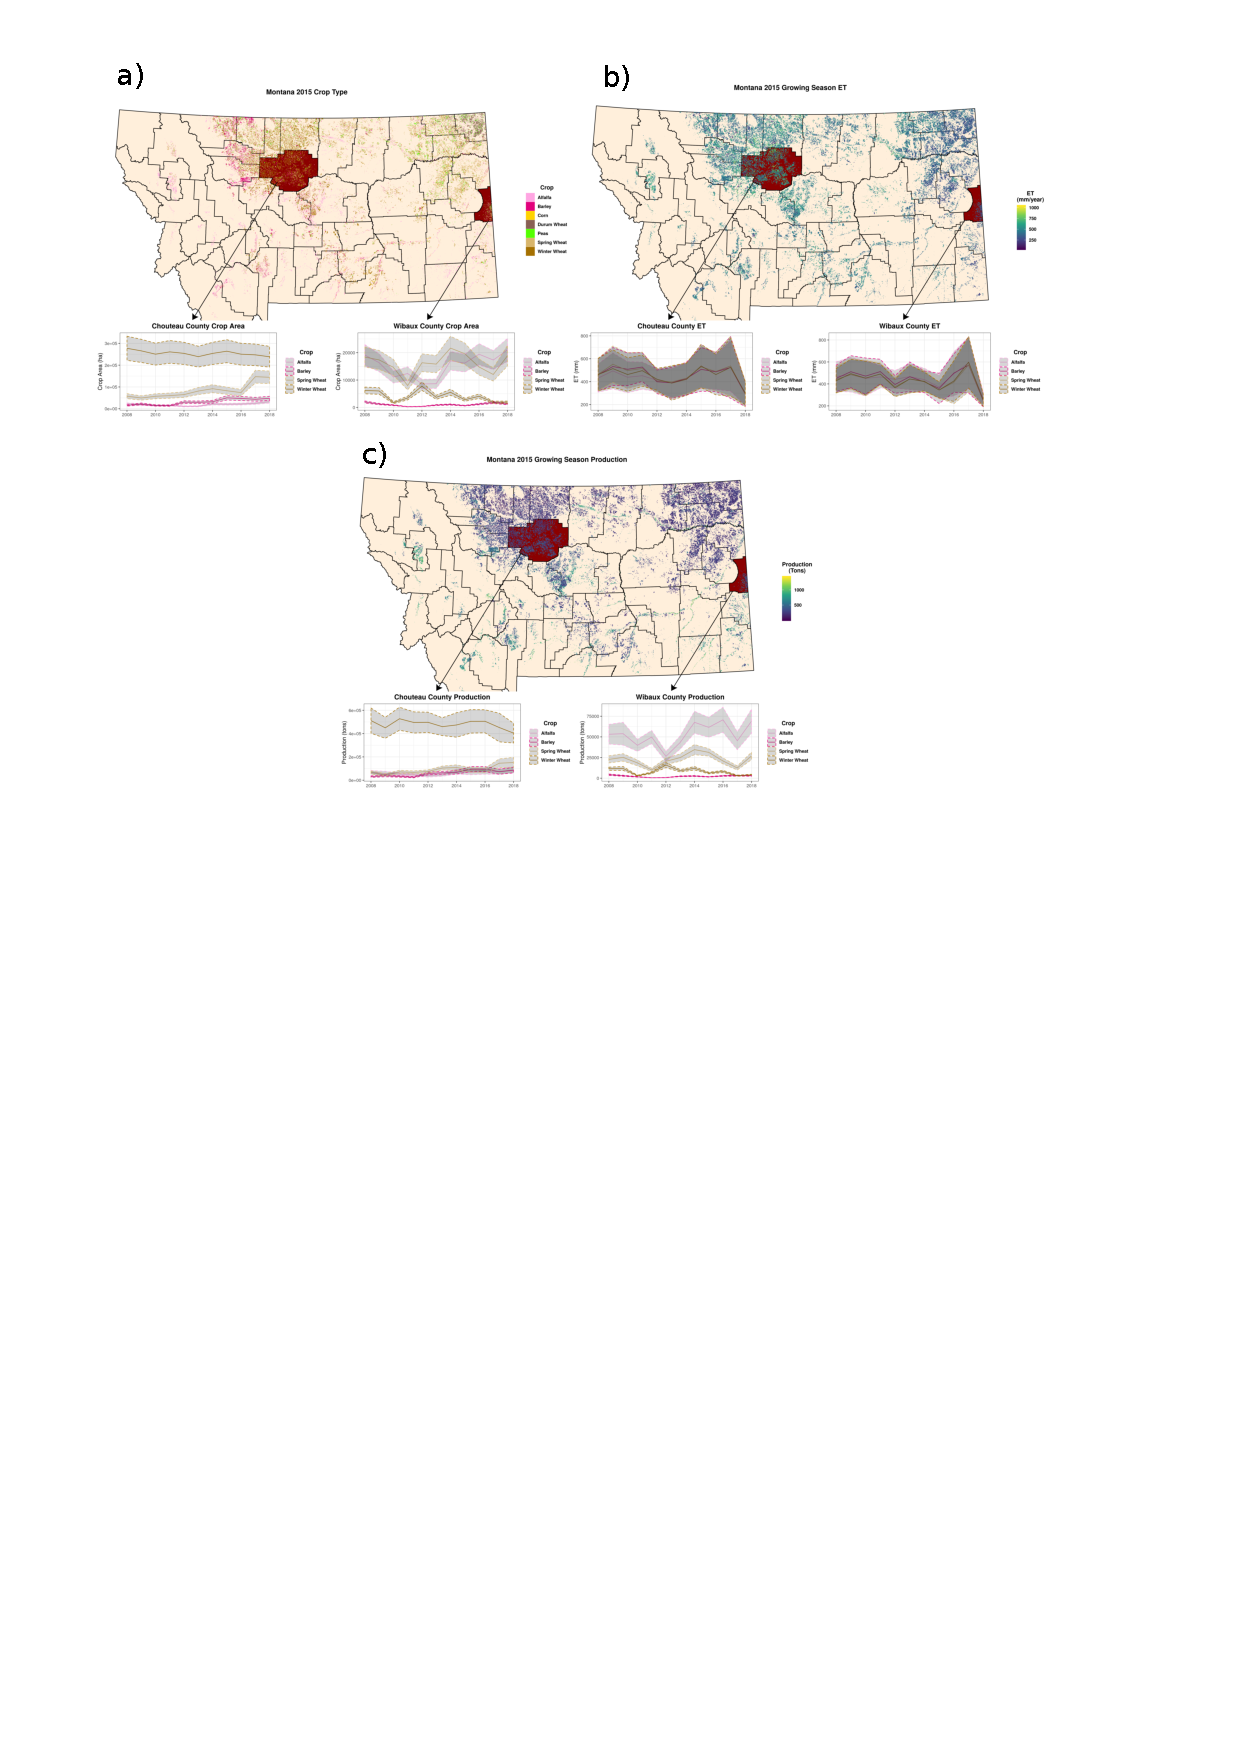
\includegraphics[width=0.8\textwidth]{MapsRemoteSensingSamples.pdf}
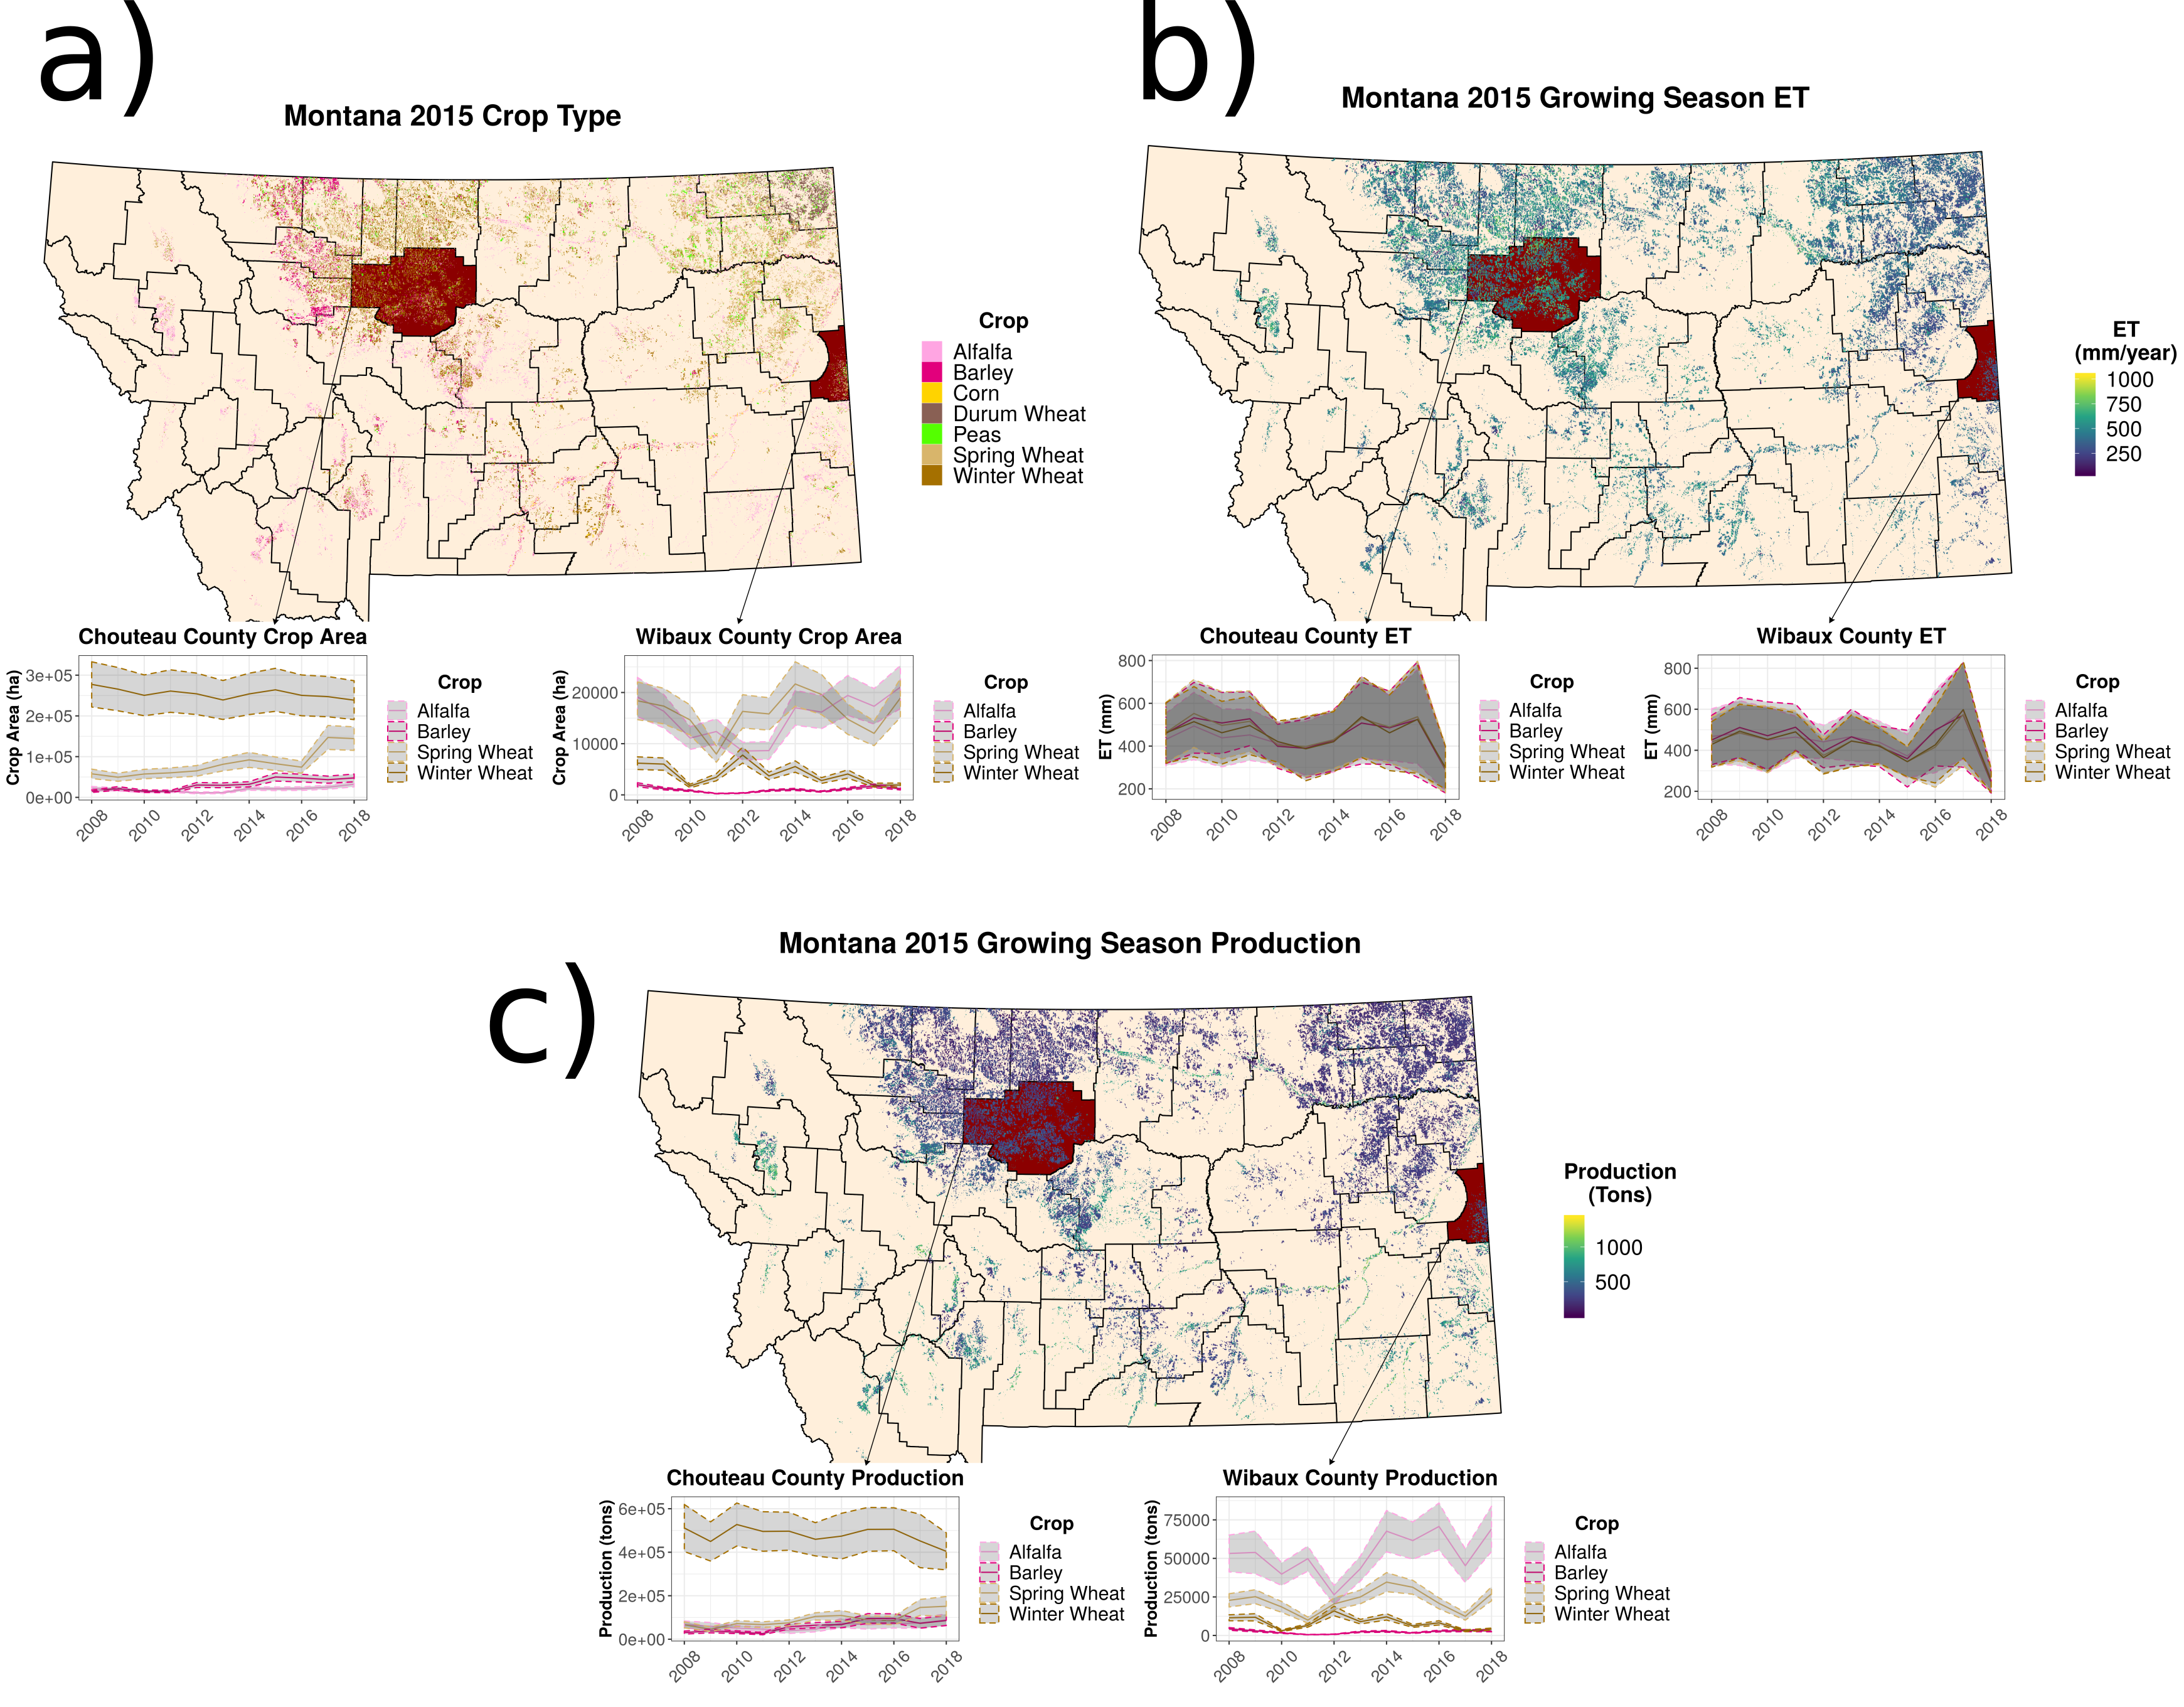
\includegraphics[width=0.9\textwidth]{Figures/RemoteSensingComposite.png}
\label{fig:crop_yield_map}
\caption{Example of remote sensing retrievals of agricultural activity over the state of Montana. The maps in the figure show pixel-level retrievals in 2009 of a) crop type, location and extent; b) seasonal crop evapotranspiration; and c) crop yield. The time series (insets) show county-aggregated variations of a) total allocated land; b) total county-level crop water use; and c) county-level total production for four example crops (alfalfa, barley, spring wheat and winter wheat) and two example counties (Choteau and Wibaux).  }
\end{figure}

Observations of crop production and yield (defined as the ratio of production to area planted) were obtained using a satellite-driven light use efficiency model to estimate gross primary production (GPP) over croplands at 30 m resolution and 8-day time step. The high spatial and temporal resolution necessary to delineate cropland vegetation growth was achieved by using a NDVI dataset that blended Landsat 5/7 reflectance and Terra MODIS reflectance. Crop yields each year were obtained by accumulating GPP over the growing season and applying a crop-specific harvest index to convert primary production to yields. \citet{He2018} gives a full description and validation of this remote sensing product. We calculated county-scale annual crop production by multiplying crop yield times the area allocated to the crop in each county. Uncertainty in the county-scale production estimates was obtained by scaling the spatial standard deviation of yields by the area planted. Figure \ref{fig:crop_yield_map}c shows an example of the 30m remotely sensed retrieved yield map and the annual variation of alfalfa, barley, spring wheat, and winter wheat production from 2009 to 2018 in two counties. 

Crop water use was estimated by adapting the operational NASA MOD16A2 global ET product \citep{Mu2011}. To better represent cropland ET our adaptation of the MOD16A2 product uses finer scale meteorological inputs from GridMet, and the same refined 30 m resolution NDVI dataset used in the estimation of production. The model parameters were also recalibrated for C3 and C4 crops. A complete description of the adaptation of MOD16A2 ET product for agricultural applications of the Conterminous US is given by \citet{He2019}. Annual variations in county-scale, crop-specific used water volumes were calculated by accumulating pixel-scale ET over the growing season and at the county scale for each crop. Uncertainty in the county-scale water use estimates was obtained by scaling the spatial standard deviation of crop ET by the area planted. Figure \ref{fig:crop_yield_map}b shows an example of the 30m remotely sensed retrieved crop ET map and the annual variation of total water volumes used by alfalfa, barley, spring wheat, and winter wheat production from 2009 to 2018 in two counties. Note that crop water use includes both evapotranspiration from precipitation and from supplemental irrigation. 

\subsection{Analysis methods}

To stabilize the model parameters with the correct values at the beginning of the analysis period we first spun up the data assimilation process by repeatedly ingesting observations from 2008 (first year in our data record) until the posterior distribution of the model parameters converged. This process optimizes the model parameters for the conditions of 2008. After the spin up was complete, we used the resulting model parameters to verify that they correctly reproduce the observed land and water allocation used to calibrate them. After this verification, we started the data assimilation process by sequentially ingesting observations from 2008 to 2016. Observations from 2017 and 2018 were available but not ingested and used to verify the the ability of the model to predict out of sample years. The model verification and analysis focused mostly on the predictions of land and water allocation, since it is one of the most novel aspect of the modeling system. However, we also demonstrated the value added by the hydrologic component by identifying the net impact of agricultural water diversions in 2017. The spatial impacts of agricultural water use were discussed qualitatively.     




\section{Results}

\subsection{Calibration and verification: parameter spin-up}

 %Write in the results that the innovations for eta and pi show that the model can reproduce observed supply elasticities and crop production 


The model parameters were spun-up to equilibrium with the conditions of 2008 (first year of the analysis period) by ingesting observations from that year during 20 assimilation cycles. The results of the parameter spin-up showed that for most counties the parameters could be accurately inferred from the assimilated observations. An example for Beaverhead county (a county with a large extent of land allocated to agriculture and also first county alphabetically) is shown in Figure \ref{fig:calibration_spinup}. Results for all counties are presented in online Appendix A. The ensemble was initiated before the spin-up with an arbitrary mean and a large spread (initial coefficient of variation of the ensemble was prescribed at 300\%) and the ensembles typically converged to a steady state distribution with very low variance within five to eight assimilation cycles. The quick convergence of the mean and the variance indicates that the observations contained sufficient information to identify the model parameters values.  Figure \ref{fig:innovation_spinup} show the dynamics of the ensemble of innovations (residual between Eq. \eqref{eq:LHS} and Eq. \eqref{eq:RHS}) for the parameter evolution of Beaverhead county shown in Figure \ref{fig:calibration_spinup}. The figure shows that, in general, the innovation quickly approached zero, which indicates that the convergence of the parameter ensembles was to a solution that satisfied the optimality conditions of the positive mathematical program (Eq. \eqref{eq:optimality_program}). The algorithm works because components (1) and (2) in Eq. \eqref{eq:LHS} represent the marginal revenues with respect to land and water allocation, and components (1) and (2) of Eq. \eqref{eq:RHS} represent the respective marginal costs. When the ensemble of differences between $LHS_i$ and $RHS_i$ is centered about zero the methodology is effectively solving the first order conditions of the net revenue maximization problem, which is the core of the calibration algorithm. Although the innovation component associated with most equations showed quick convergence, some of them, such as component (2) of the innovation for irrigated spring wheat or for irrigated alfalfa in Beaverhead county, converged to a nonzero value. Biases in component (2) of the innovation indicate that the parameter ensemble of $\lambda_{water}$ converged to a suboptimal value. Online Appendix B shows the evolution of the innovation ensembles associated with the parameter spin-ups in all counties in the state of Montana.    

\begin{figure}
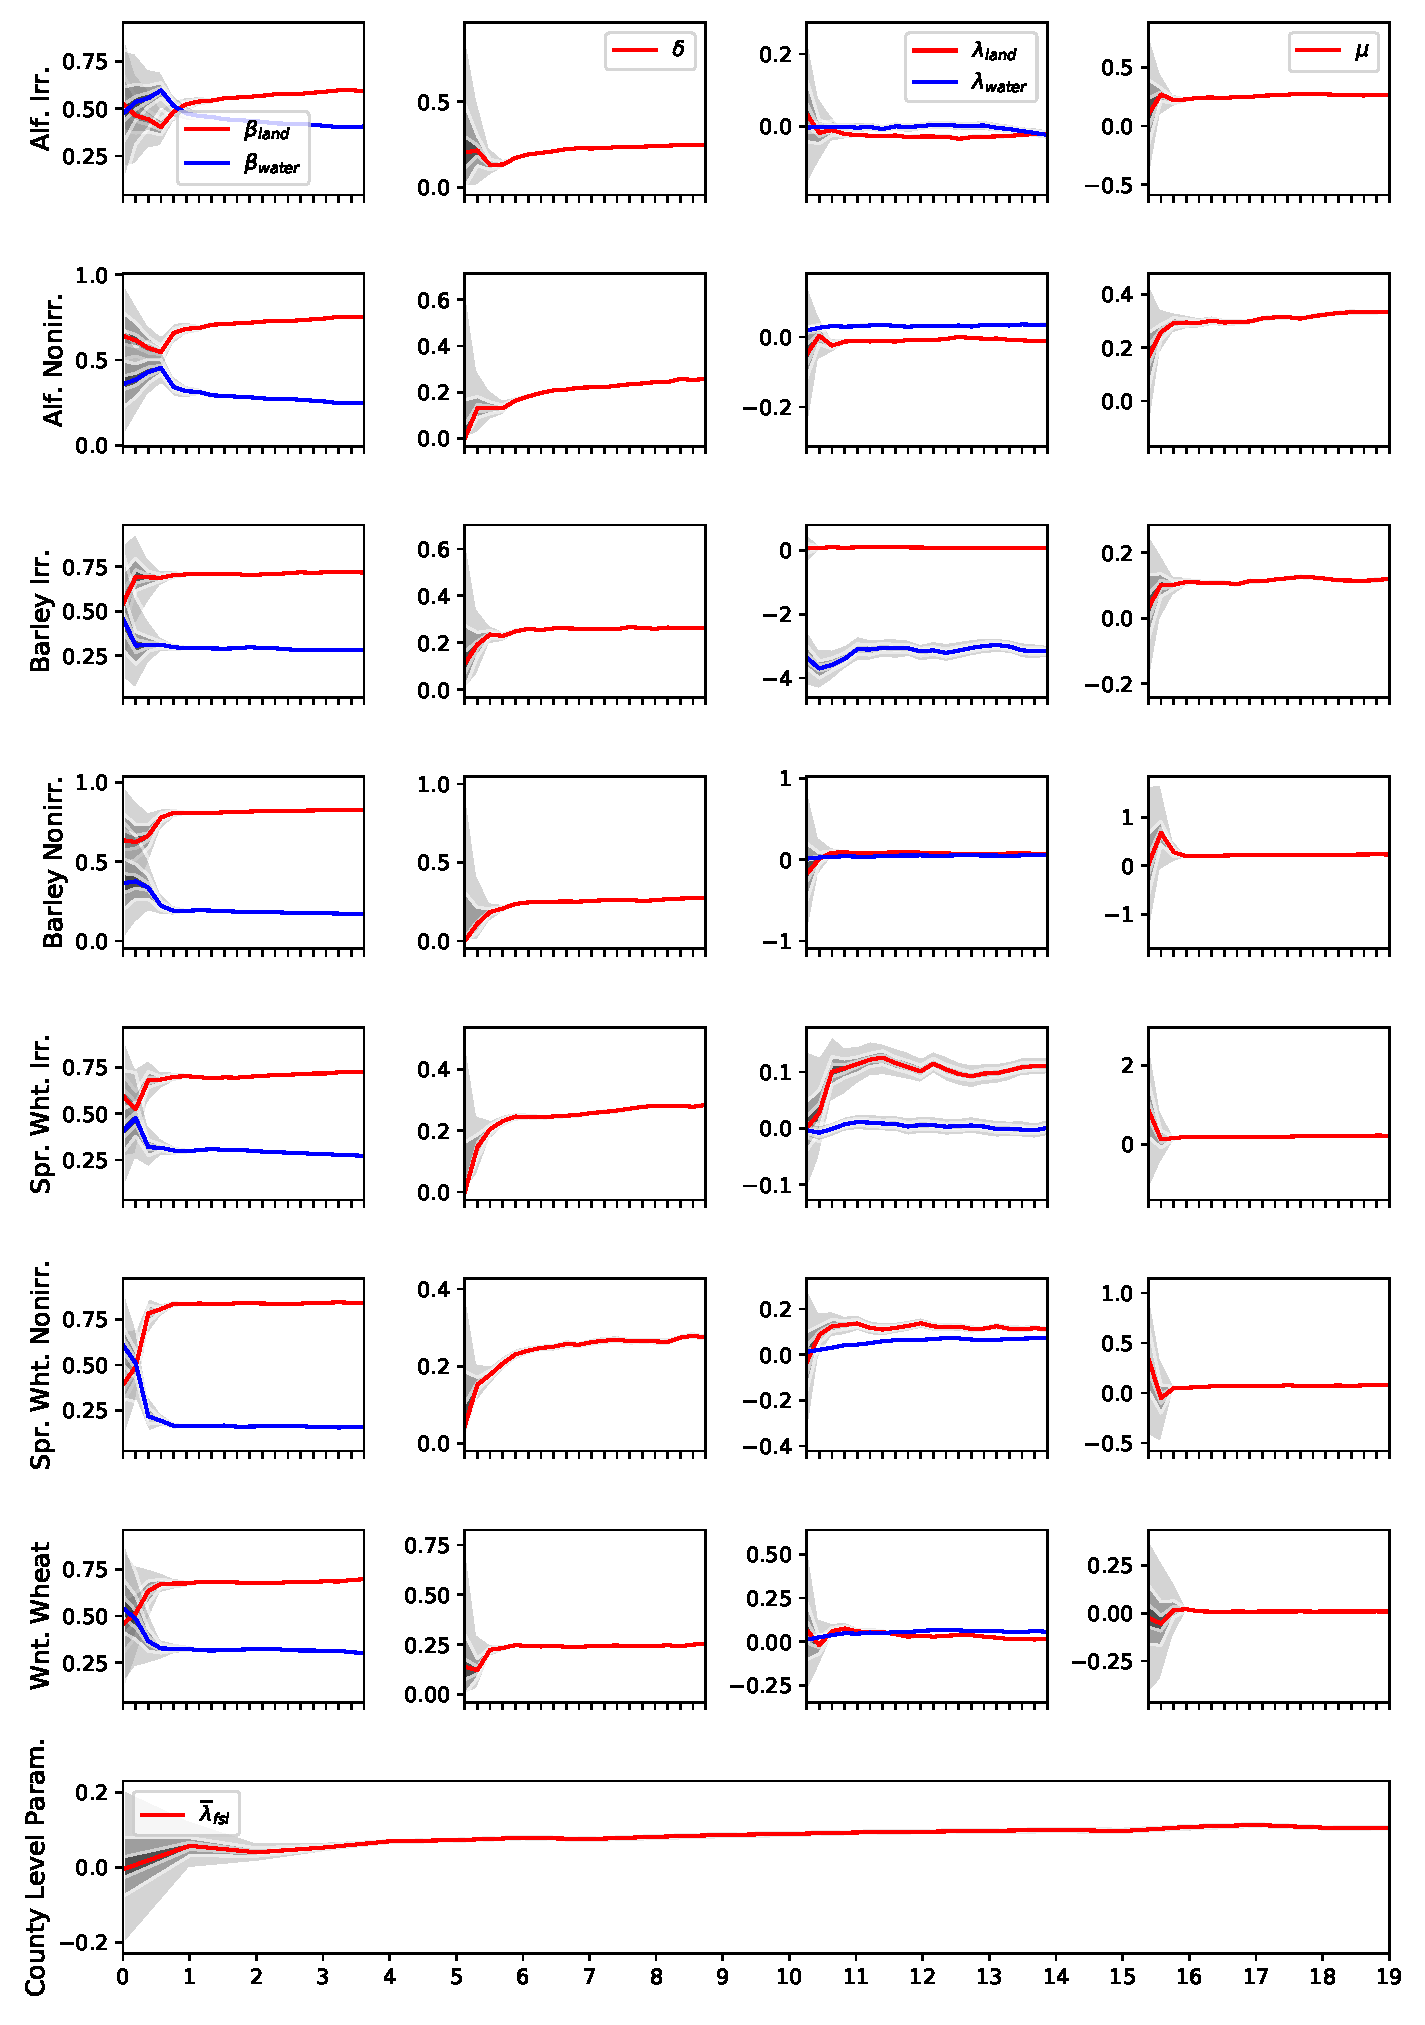
\includegraphics[width=0.8\textwidth]{Figures/cal_spin_Beaverhead.pdf}
\label{fig:calibration_spinup}
\caption{Evolution of the parameter ensemble during parameter spin-up in Beaverhead county. Shaded areas are the 95 and 68 percentile confidence intervals of the ensemble. Ensembles for all counties is presented in online Appendix A}
\end{figure}


\begin{table}[]
\resizebox{0.8\textwidth}{!}{%
\centering
\begin{threeparttable}
\caption{Mean relative bias (Rel. Bias \tnote{a}) and relative root mean square error (Rel. RMSE\tnote{b}) statistics for the simulation land allocated during the 2008 benchmark conditions. }
\label{tab:gof_spinup}

\begin{tabular}{|l|l|l|l|l|}
\hline
                          & \multicolumn{4}{c|}{2018}                                                         \\ \hline
                          & \multicolumn{2}{c|}{Land Use}           & \multicolumn{2}{c|}{Water Use}          \\ \hline
                          & \textit{Rel. Bias} & \textit{Rel. RMSE} & \textit{Rel. Bias} & \textit{Rel. RMSE} \\ \hline
Alfalfa Irrigated         & -0.062             & 0.142              & -0.172             & 0.257              \\ \hline
Alfalfa Nonirrigated      & -0.021             & 0.08              & -                  & -                  \\ \hline
Barley Irrigated          & 1.826              & 1.939             & 2.694208           & 1.125              \\ \hline
Barley Nonirrigated       & -0.020             & 0.018              & -                  & -                  \\ \hline
Spring Wheat Irrigated    & -0.028             & 0.138              & 0.715453           & 1.00               \\ \hline
Spring Wheat Nonirrigated & -0.020             & 0.014              & -                  & -                  \\ \hline
Winter Wheat              & -0.019             & 0.062              & -                  & -                  \\ \hline
\end{tabular}%

\begin{tablenotes}\footnotesize
\item [a] $Rel. Bias = \frac{sim_i - obs_i}{obs_i}$
\item [b] $Rel. RMSE = \frac{\sqrt{\frac{1}{n}\sum_i^n(sim_i - obs_i)^2}}{\frac{1}{n}\sum_i^n obs_i}$
\end{tablenotes}
\end{threeparttable}
}
\end{table}


The ensemble of parameters obtained at the end of the spin-up cycle was used to predict the land and water allocation for the 2008 baseline. Although the ensemble of innovations indicate that some parameter distributions converge to suboptimal values, the model was able predict land and water allocations with satisfactory accuracy, as summarized in Table \ref{tab:gof_spinup}. The correlation coefficient between county-wise simulated and observed land allocation is higher than 0.98 and the relative bias of the estimation is typically less than 0.06 (6\%). The exception are the simulation of land allocated to irrigated barley, which showed significantly lower correlation and higher bias than the other crops.         

\begin{figure}
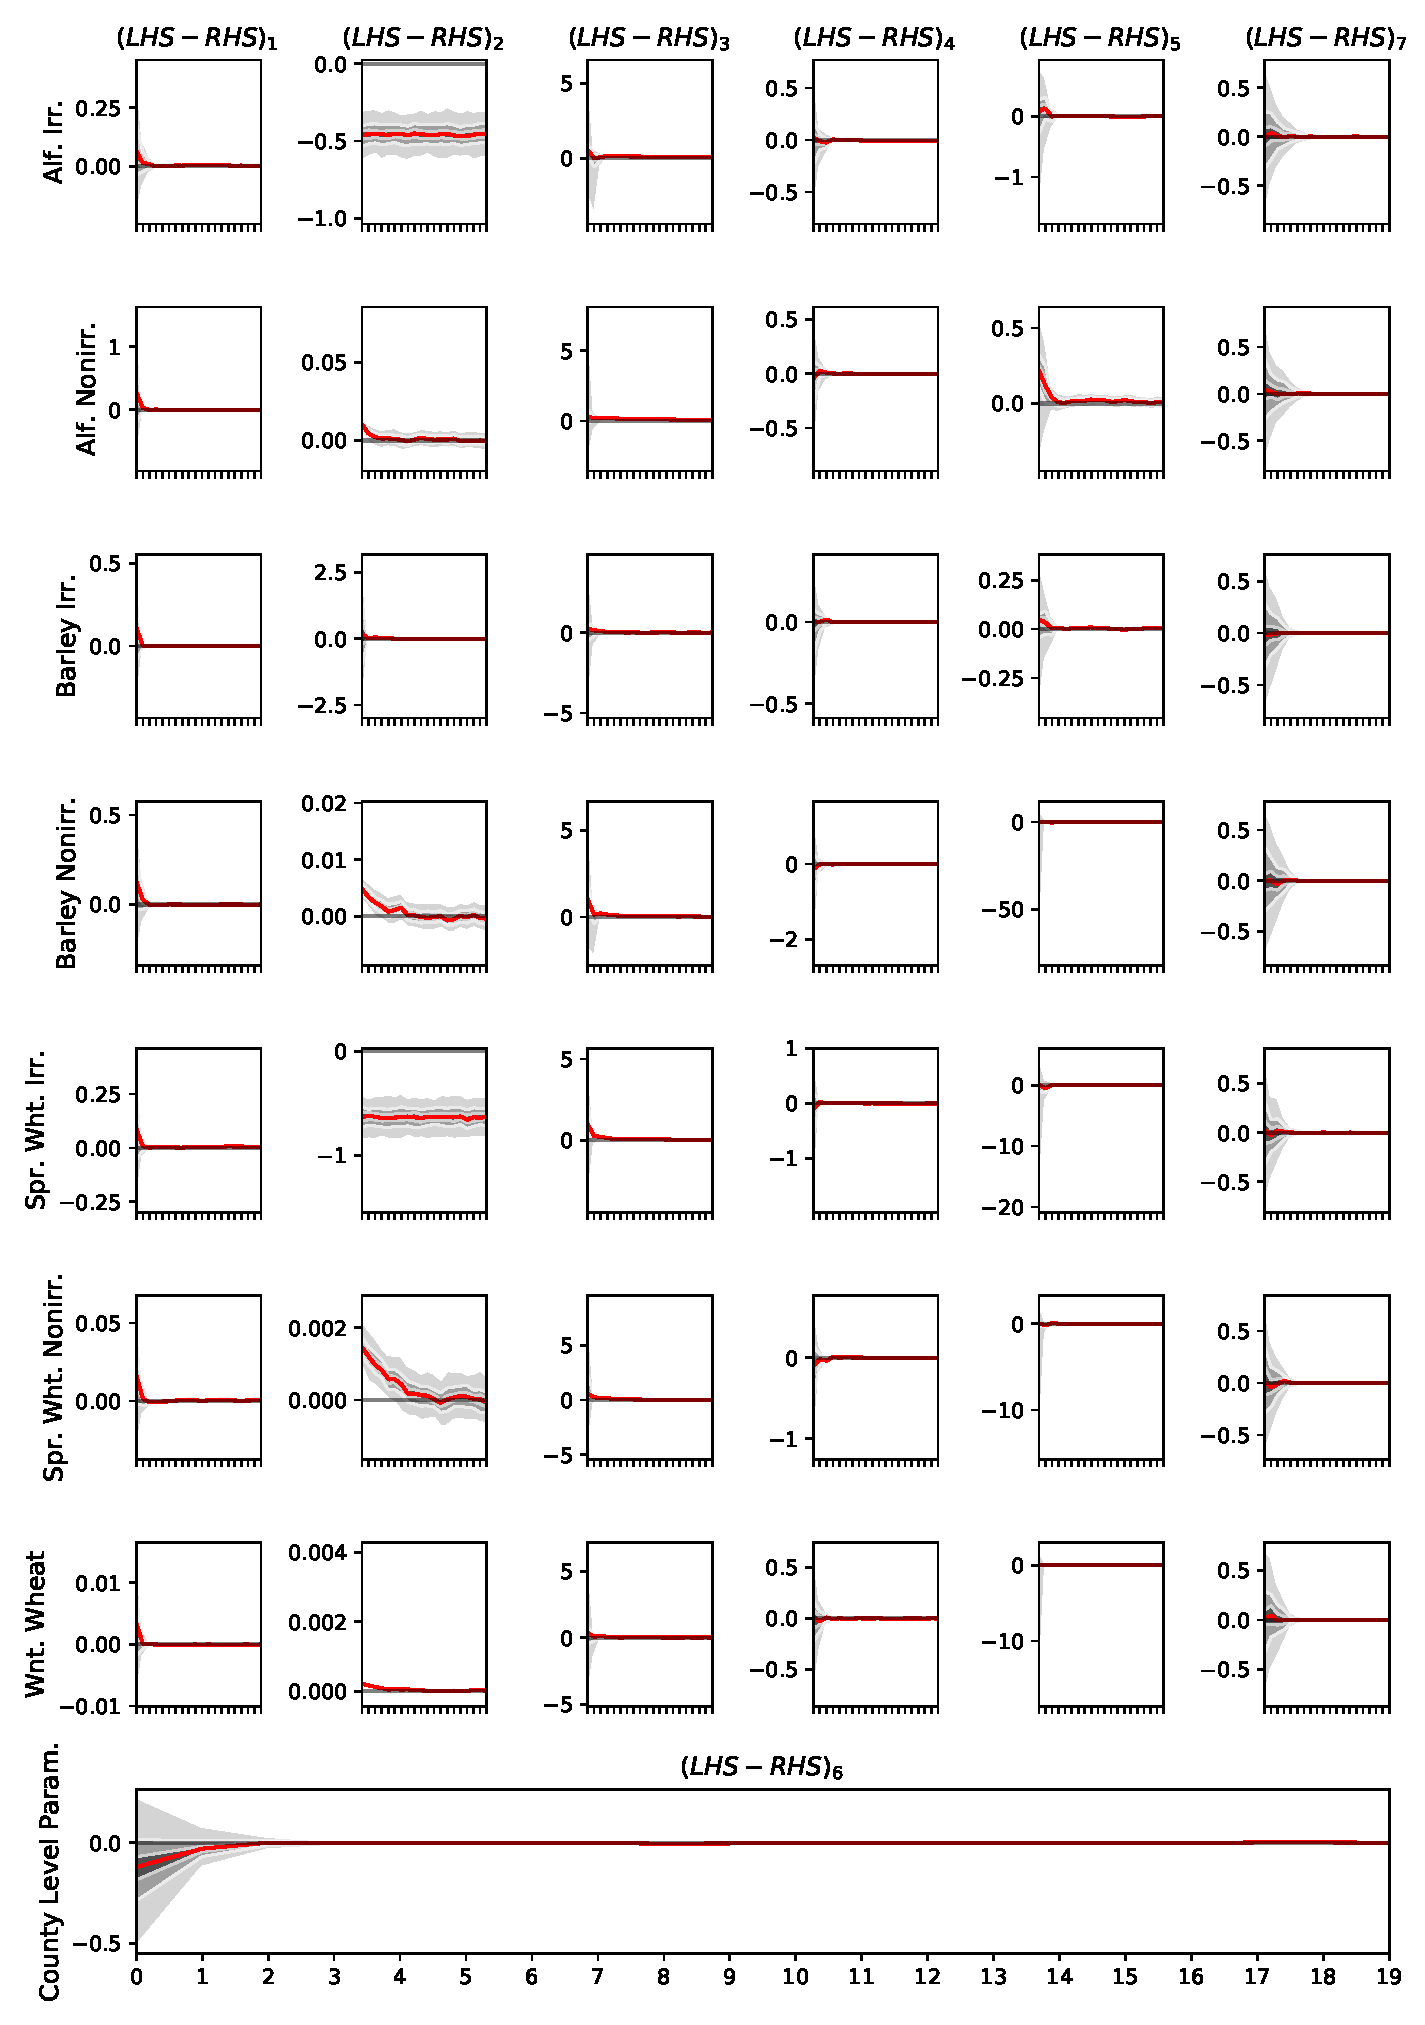
\includegraphics[width=0.8\textwidth]{Figures/inn_spin_Beaverhead.pdf}
\label{fig:innovation_spinup}
\caption{Evolution of the filter innovation during parameter spinup corresponding to the ensembles in Figure \ref{fig:calibration_spinup}. Subscript of column titles refer to a innovation component as numbered in Eqs. \eqref{eq:LHS} and \eqref{eq:RHS}. Shaded areas are the 95 and 68 percentile confidence intervals of the ensemble. Ensemble for all counties is presented in online Appendix B}
\end{figure}

A comparison between the predicted probability distributions of land and water allocation and actual allocations provides a direct evaluation of the model predictive skills for individual counties and also illustrates how parameter uncertainty translates into uncertainty in the predictions of resource allocation. Figure \ref{fig:hist_land_alloc} shows the simulated probability distribution of land allocated to the crops grown in Beaverhead county along with the observed allocation. Online appendix C shows the simulated land allocation for all crops and counties. In general, for most counties and crops, the predictive distributions are well centered around the observation or bracket the observations within the high probability density interval. The probability distribution of the predictions reflect the sensitivity of predictions to the spread of the parameter ensemble.  

\begin{figure}
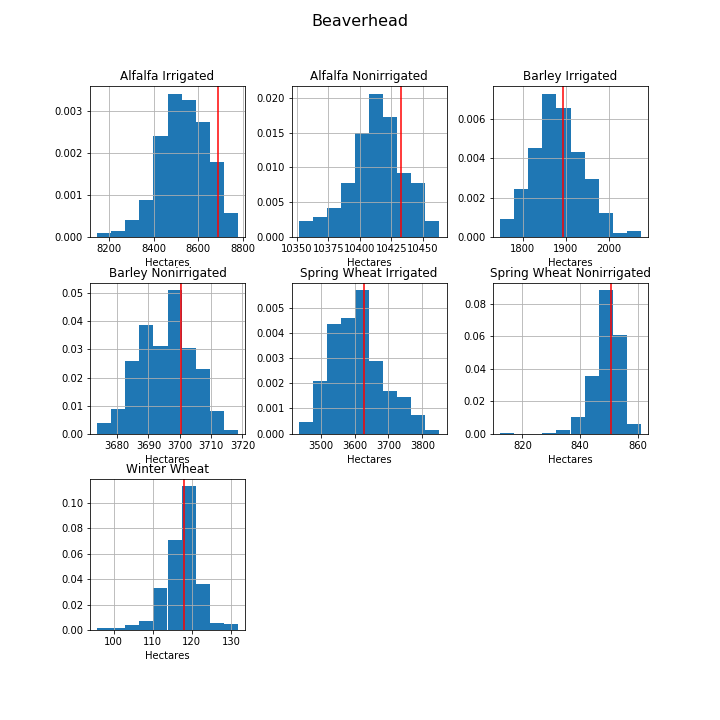
\includegraphics[width=0.8\textwidth]{Figures/30001_hist_2008.png}
\label{fig:hist_land_alloc}
\caption{Simulated probability distributions (blue bars) and observed (red lines) land allocation in 2009 for seven crops grown in Beaverhead county, MT. Simulations for all counties is presented in online Appendix C.}
\end{figure}

Comparison between observed and modeled water allocation for irrigation is less straightforward because water allocation per crop and county is not directly observed. Remote sensing ET observations only provide total crop water use, which integrates water from natural precipitation and from supplemental irrigation. However, the simulation scenarios require that the the expected amount of water from natural sources used by crops (natural ET) is specified.  However, the simulation scenarios require that the the expected amount of water from natural sources used by crops (natural ET) is specified. Subtracting this specified natural ET amount from the total observed crop water use gives us an estimate of the amount of crop water use supplemented by irrigation. This estimate served as the observation of supplemental irrigation used to evaluate the model simulation of water allocation.  Figure \ref{fig:hist_water_alloc} shows the case of Beaverhead county. Figures for water allocation in all counties in the state are provided in online appendix D. Similar to the simulation of land use, the simulation of water allocation per crop and county is also centered around the observations, bracketing them in most cases within the high probability region of predictions.   

\begin{figure}
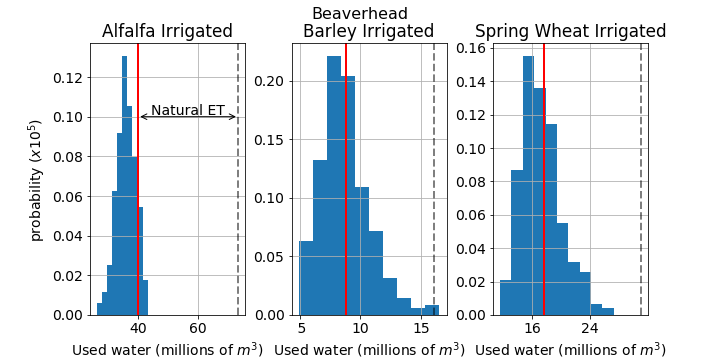
\includegraphics[width=0.6\textwidth]{Figures/30001obs_water_hist_2008.png}
\label{fig:hist_water_alloc}
\caption{Simulated probability distribution of water allocation for three irrigated crops grown in Beaverhead county, MT (blue bars). Dashed grey vertical line indicates the observed total evapotranspiration consumed by the crop (evaporation from natural supplies and from supplemental irrigation). Benchmark supplemental irrigation (red vertical line), was estimated by subtracting water used by crops from natural supplies  (natural ET) as prescribed in the modeled scenario from the observed total crop evapotranspiration. Simulations for all counties is presented in online Appendix D.}
\end{figure}

\subsection{Dynamics of the parameter ensemble}

Using the parameter distributions obtained at the end of the spin-up period as a starting point, we assimilated remote sensing observations from 2009 through 2016. Figure \ref{fig:calibration2008-2015} shows the dynamics of the parameter ensembles for Beaverhead county over the the eight years of data assimilation. Note that the $y$ axis has been re-scaled with respect to that of Figure \ref{fig:calibration_spinup} to better represent the ensemble spread. Figures for all counties are available in online appendix E. In general, parameters $\beta_{land}$ and $\beta_{water}$ showed very high stability and very little dispersion over time, with very small drifts in their mean value. To a lesser degree, parameter $\delta$ also presented relatively high stability and low ensemble dispersion. On the other hand, $\lambda_{land}$, $\lambda_{water}$, and the $\mu$ parameters showed large ensemble dispersion and high sensitivity to variations in the input observations. The evolution of the parameters sometimes exhibited smooth drifts over the data assimilation period (e.g. parameter $\mu$ for non-irrigated spring wheat non-irrigated in Figure \ref{fig:calibration2008-2015}), sudden realignments after a specific year (e.g. the case of $\lambda_{land}$, $\lambda_{water}$ for winter wheat and $\overline{\lambda}_{fsl}$ in year 2010), or fluctuations about a long term mean without a clear trend (e.g. parameter $\mu$ for winter wheat in Figure \ref{fig:calibration2008-2015})).


\begin{figure}
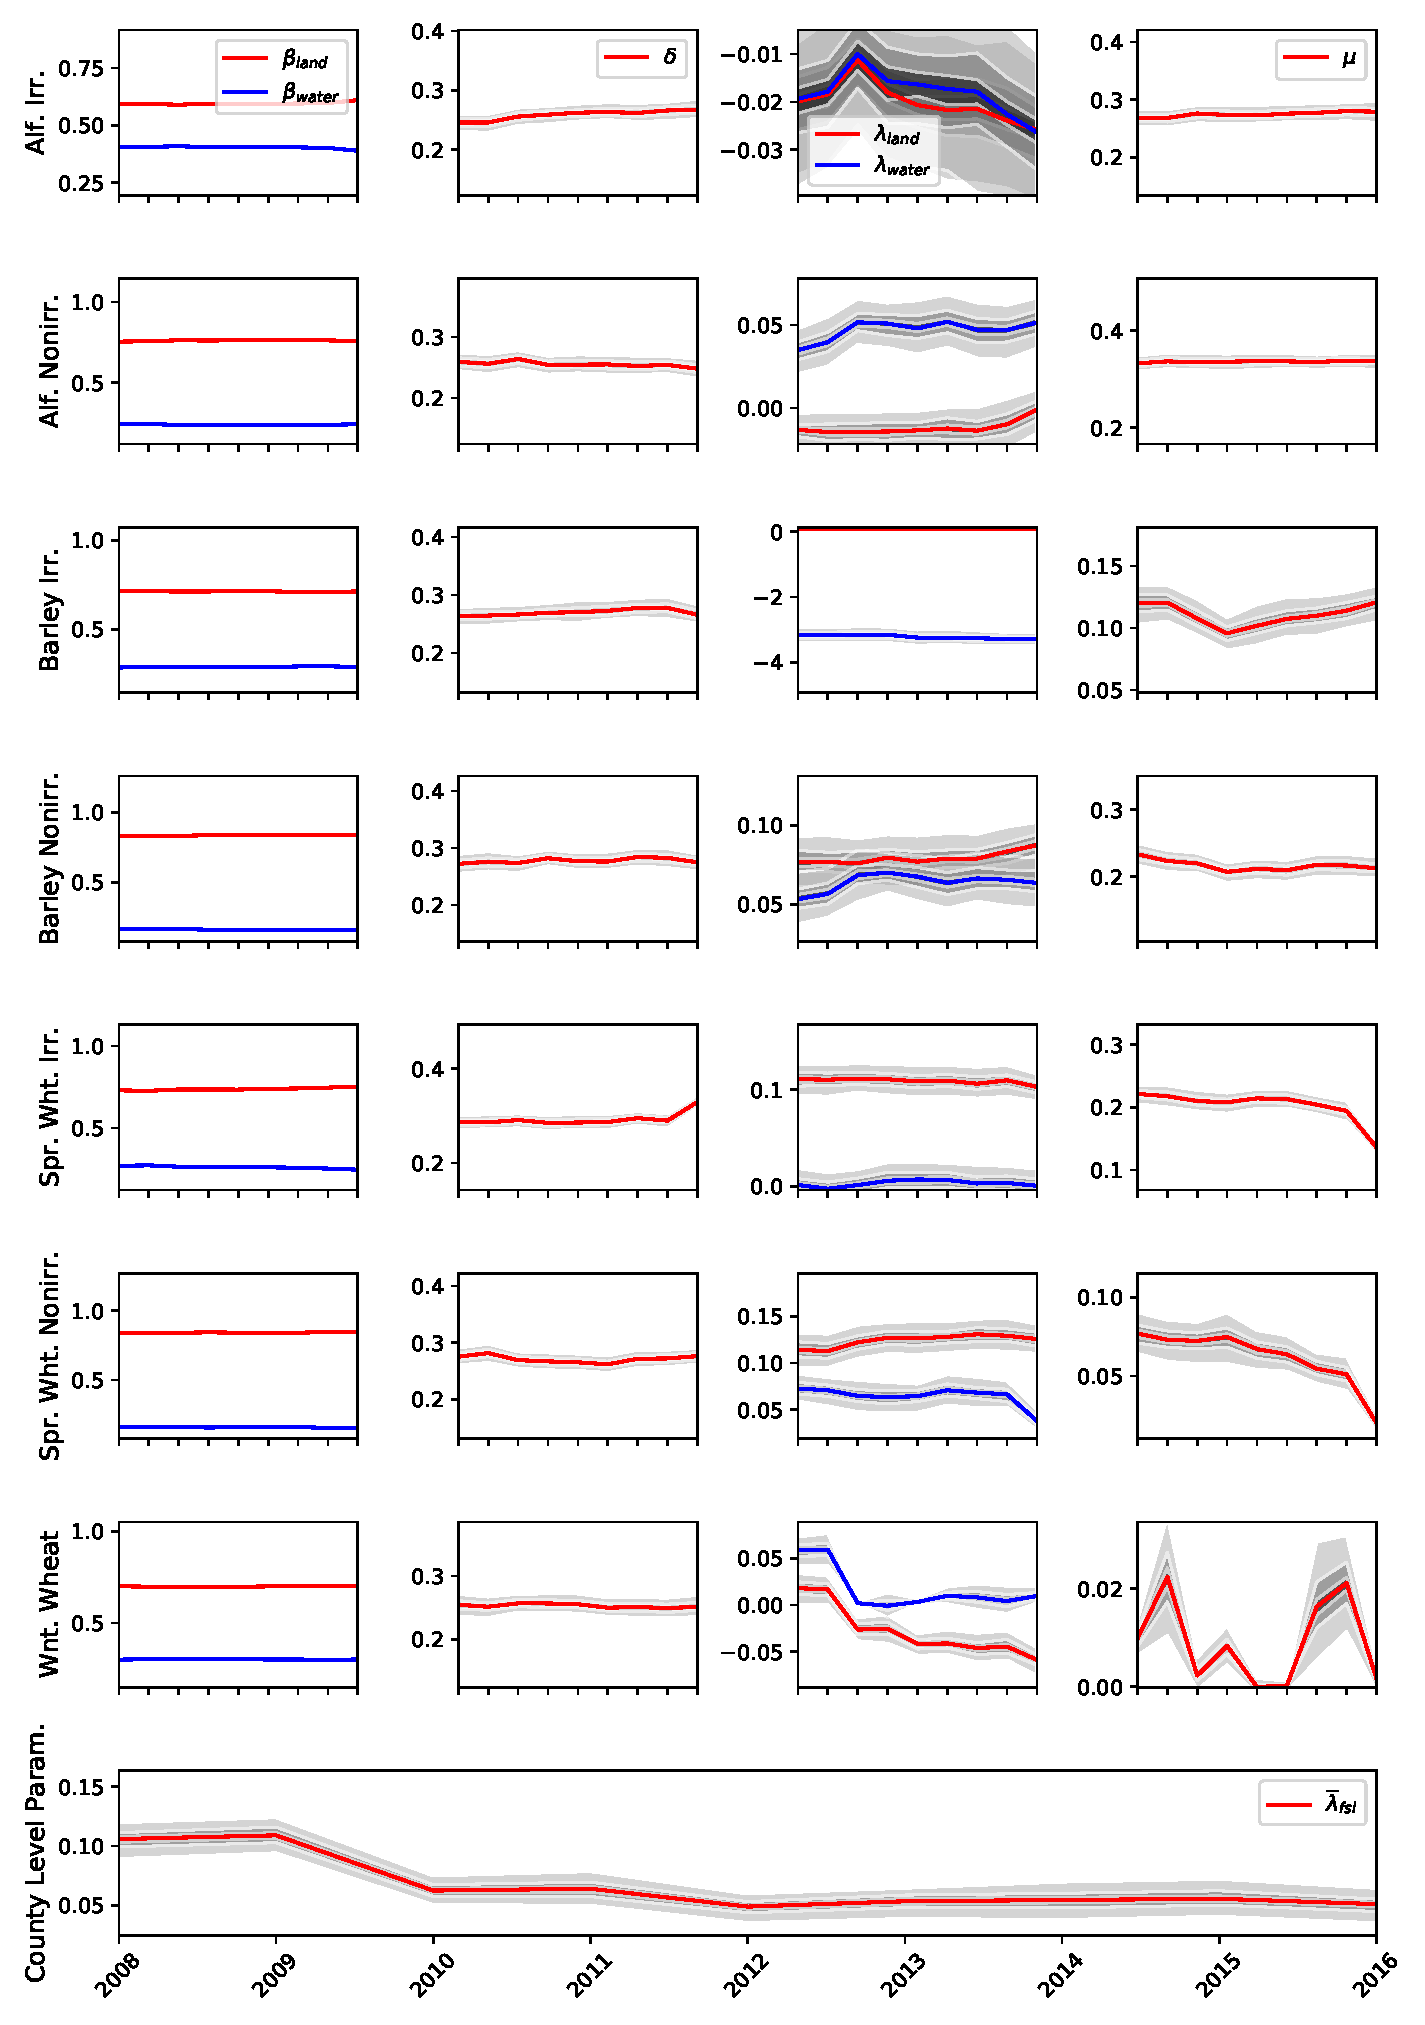
\includegraphics[width=0.8\textwidth]{Figures/cal_Beaverhead.pdf}
\label{fig:calibration2008-2015}
\caption{Dynamics of the parameter ensembles over 8 years (2008-2016) of data assimilation in Beaverhead county. Parameters start from the distribution achieved at the end of the spin-up period in 2008. Shaded areas are the 95 and 68 percentile confidence intervals of the ensemble. Figures for all other counties are presented in Online Appendix E. }
\end{figure}

The dynamics of the innovation associated with the parameter ensembles in Fig.\ref{fig:calibration2008-2015} were in general tightly centered around zero for most components, reflecting the precision and accuracy with which the parameters can be tracked over time (Figure \ref{fig:innovation20082015}). The filter maintained most of the parameters at optimal values and indicated that the model was ready for operational use throughout the assimilation period. The exception to this was component (2) of the innovation, which showed high variance and a significant bias for alfalfa and irrigated winter wheat. Although Figure \ref{fig:innovation20082015} represents the case of Beaverhead county, component (2) of the innovation was often the one that exhibited the largest amount of bias and variance over all counties. This component of the innovation is controlled by parameter $\lambda_{water_i}$, which was shown in Fig. \ref{fig:calibration2008-2015} to be the least identifiable parameter.  

%The evolution of the parameters is required to meet the optimality conditions embedded in the filter, however the equation that describes the artificial evolution of the parameters (Eq. \eqref{eq:param_evolution}) contains a smoothing factor that controls the sensitivity of the parameter ensemble to new information. Damping the response of the parameters to observations makes their dynamics more stable but also can generate suboptimal innovations.




\subsection{Simulation of years 2017 and 2018}

Table \ref{tab:gof} shows the relative bias and root mean square relative error (RMSRE) of the mean predicted vs observed crop acreage and water allocation over all counties in Montana for years 2017 and 2018. For these simulations, the model was run with the parameter distribution obtained at the end of the 2008-2016 assimilation period. For most crops, the simulation of the 2017 land and water use showed a higher bias and RMSRE than in 2018. This larger model predictive error in 2017 is associated with the abnormal conditions generated by the severe flash drought that affected the US Northern Plains in the summer of 2017 \citep{He2019, Kimball2019}.  Despite the better predictive performance of the model in 2018, the results for the two simulated years are qualitatively very similar and therefore we only present and discuss the predictions for year 2017. The discussion of the results from 2017 also apply to the simulations of year 2018.        

\begin{figure}
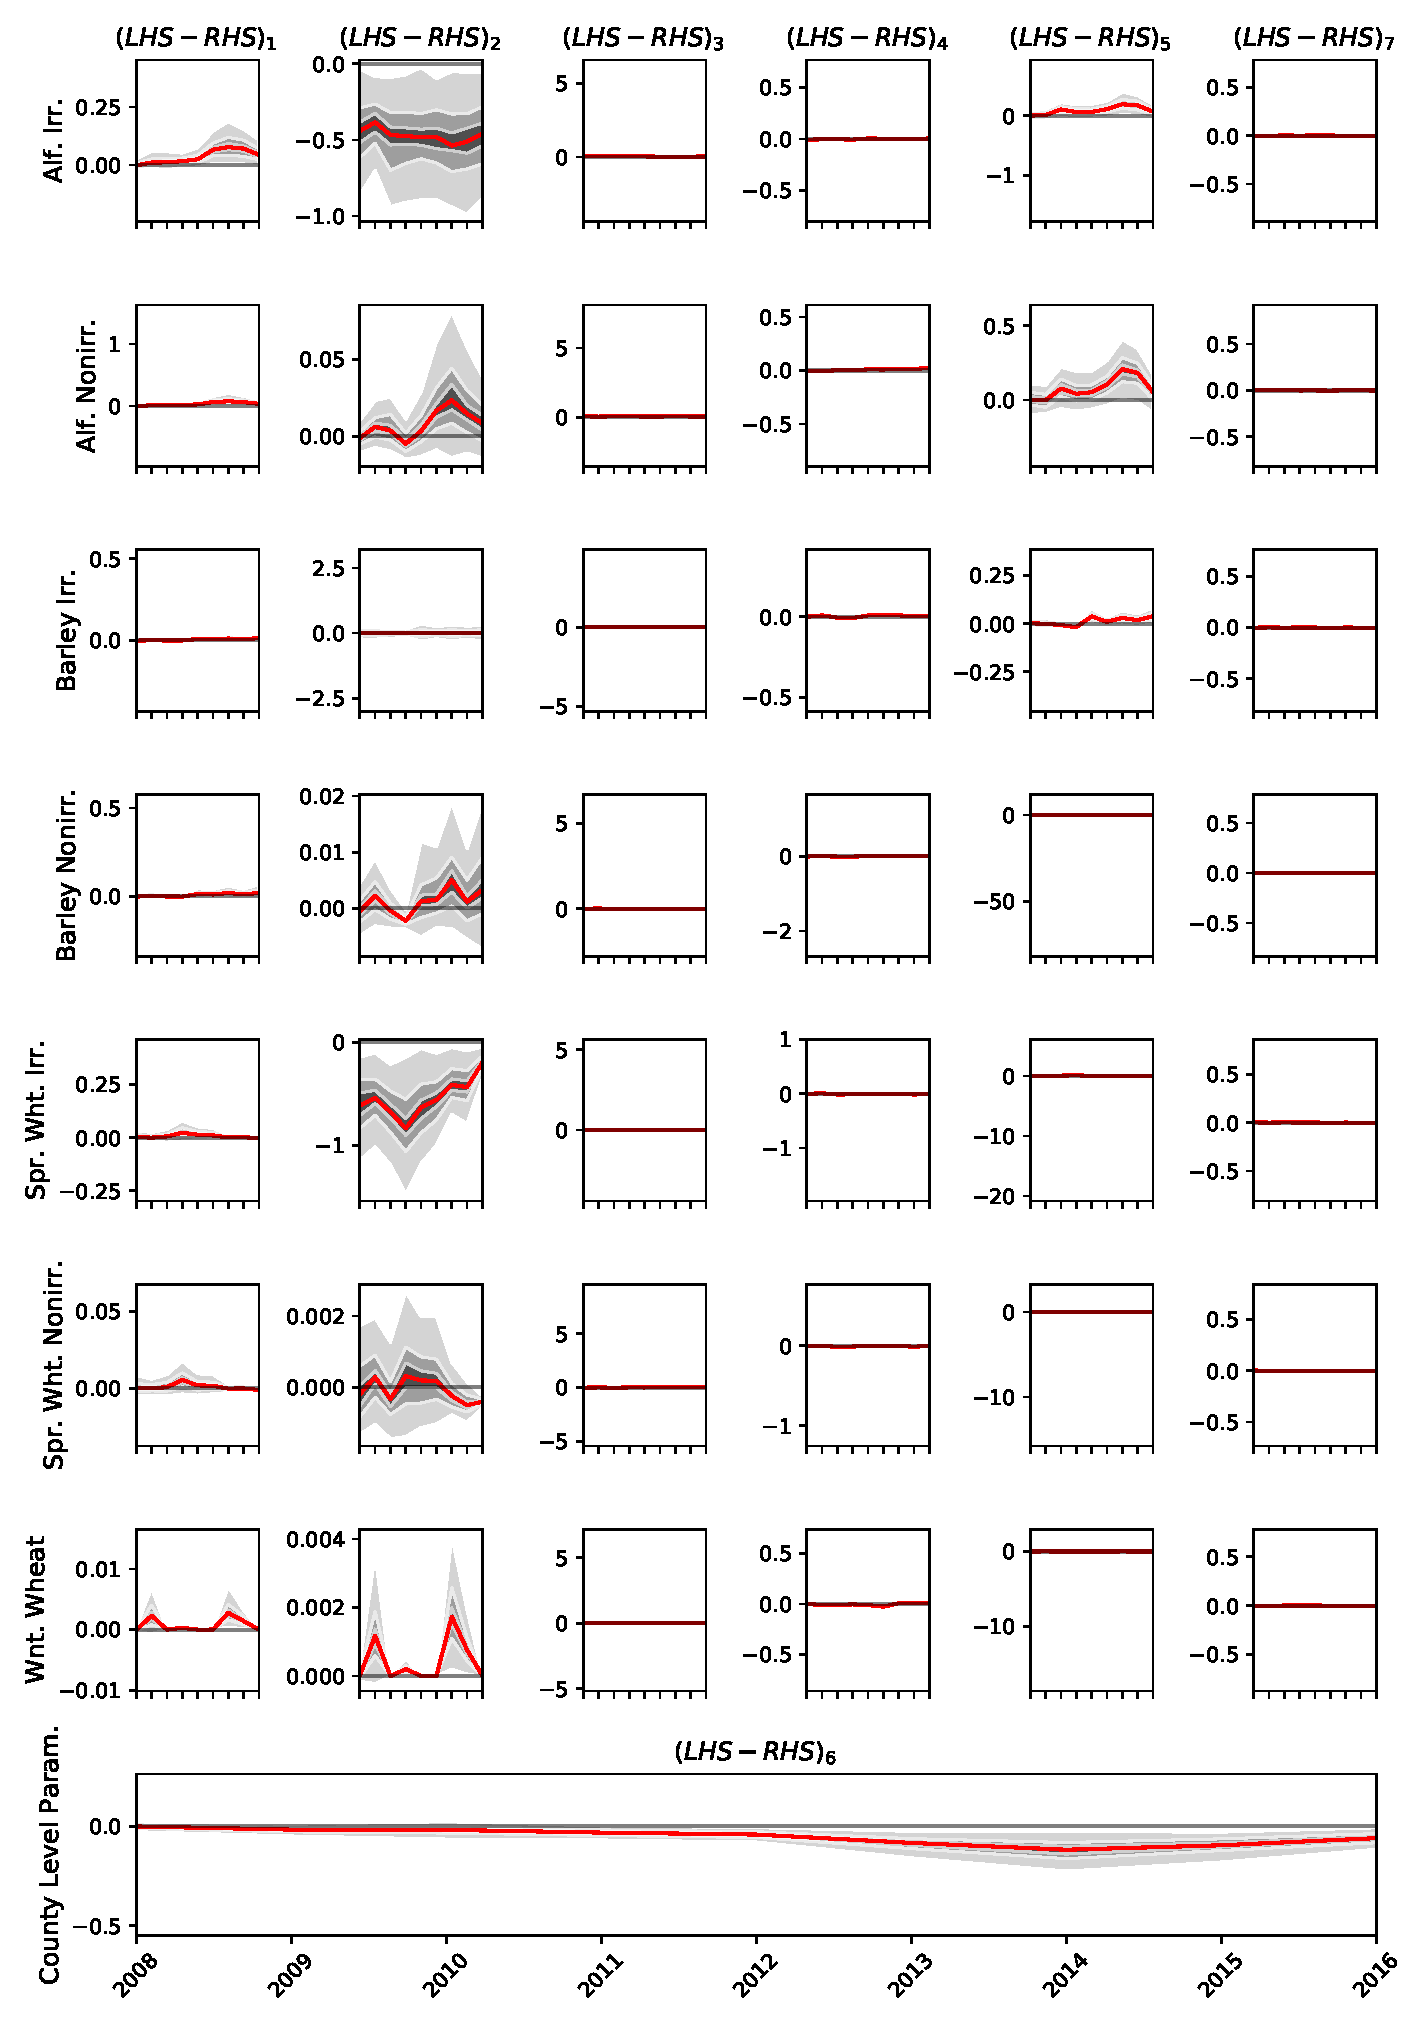
\includegraphics[width=0.8\textwidth]{Figures/figure_Beaverhead.pdf}
\label{fig:innovation20082015}
\caption{Dynamic of the innovation over 8 years (2008-2015) of assimilation corresponding to the parameter ensembles shown in Figure \ref{fig:calibration_spinup}. Subscript of column titles refer to a innovation component as numbered in Eqs. \eqref{eq:LHS} and \eqref{eq:RHS}. Shaded areas are the 95 and 68 percentile confidence intervals of the ensemble. Ensemble for all counties is presented in online Appendix F}
\end{figure}

% Please add the following required packages to your document preamble:
% \usepackage{graphicx}
\begin{table}[]
\resizebox{0.8\textwidth}{!}{%
\centering
\begin{threeparttable}
\caption{Mean relative bias (Rel. Bias \tnote{b}) and relative root mean square error (Rel. RMSE \tnote{b}) statistic for the simulation of land allocation and water allocation under the conditions of years 2017 and 2018.}
\label{tab:gof}

\begin{tabular}{|l|l|l|l|l|l|l|l|l|}
\hline
                          & \multicolumn{4}{c|}{2017}                                      & \multicolumn{4}{c|}{2018}                                      \\ \hline
                          & \multicolumn{2}{c|}{Land use} & \multicolumn{2}{c|}{Water use} & \multicolumn{2}{c|}{Land use} & \multicolumn{2}{c|}{Water use} \\ \hline
 &
  \textit{Rel. Bias} &
  \textit{Rel. RMSE} &
  \textit{Rel. Bias} &
  \textit{Rel. RMSE} &
  \textit{Rel. Bias} &
  \textit{Rel. RMSE} &
  \textit{Rel. Bias} &
  \textit{Rel. RMSE} \\ \hline
Alfalfa Irrigated         & -0.003         & 0.151        & -0.172         & 0.805         & -0.067         & 0.182        & -0.104         & 0.542         \\ \hline
Alfalfa Nonirrigated      & 0.155          & 0.277        & -              & -             & -0.045         & 0.133        & -              & -             \\ \hline
Barley Irrigated          & 0.319          & 0.305        & 2.694          & 3.09          & -0.193         & 0.379        & 5.745          & 3.135         \\ \hline
Barley Nonirrigated       & 0.301          & 0.476        & -              & -             & -0.155         & 0.226        & -              & -             \\ \hline
Spring Wheat Irrigated    & 1.321          & 0.540        & 0.715          & 2.511         & 2.531          & 0.508        & 0.419          & 2.05          \\ \hline
Spring Wheat Nonirrigated & -0.005         & 0.285        & -              & -             & -0.037         & 0.165        & -              & -             \\ \hline
Winter Wheat              & -0.241         & 0.488        & -              & -             & -0.167         & 0.089        & -              & -             \\ \hline
\end{tabular}%
\begin{tablenotes}\footnotesize
\item [a] $Rel. Bias = \frac{sim_i - obs_i}{obs_i}$
\item [b] $Rel. RMSE = \frac{\sqrt{\frac{1}{n}\sum_i^n(sim_i - obs_i)^2}}{\frac{1}{n}\sum_i^n obs_i}$
\end{tablenotes}
\end{threeparttable}
}
\end{table}

The model satisfactorily reproduced the county-scale distribution of cropping patterns (Figure \ref{fig:map_land_change}). Alfalfa is grown in all states and the model predictions capture well the spatial distribution of land allocation for this crop (Figure \ref{fig:map_land_change} rows 1 and 2). Note that the area planted with non-irrigated alfalfa tends to be larger in the eastern third of the state because that region is characterized by large properties and extensive ranching. This distribution is well captured in the model predictions. On the other hand, irrigated alfalfa is more common in the southern and southwest portions of the state, in counties close to the border with Wyoming and in the upstream end of the Gallatin, Yellowstone and Missouri rivers. This is also correctly captured by the model. Also remarkable is the ability of the model to identify the regions in the state that specialize in small grain production. The model correctly identifies the counties in the west and north west central region of Montana that allocate the most land to irrigated and non-irrigated barley (Figure \ref{fig:map_land_change} rows 3 and 4). It also identifies very well the swath of counties in the north and north east portions of the state that allocate the most land to grow spring wheat and winter wheat (Figure \ref{fig:map_land_change} rows 5 and 6). The spatial distribution of relative errors show some complex spatial patterns, but in general relative errors in simulated area allocated to a crop are largest in counties where observations of area planted with a given crop are small because relative errors are normalized by these observations. This causes the summary statistics presented in Table \ref{tab:gof} to be skewed by very large errors in a small number of counties. This is particularly evident in the statistics of land allocated to irrigated barley and irrigated spring wheat, where simulated land allocation tends to underestimate observations (negative relative errors represented by blue colors in Figure \ref{fig:map_land_change}), but Table \ref{tab:gof} reports a large positive relative bias.     
 
\begin{figure}
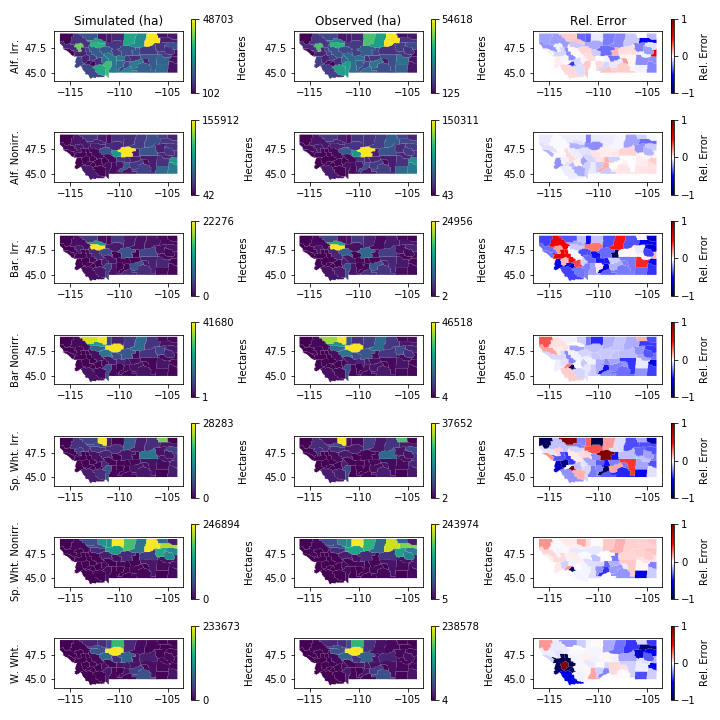
\includegraphics[width=\textwidth]{Figures/mean_land_use_2018.png}
\label{fig:map_land_change}
\caption{Comparison between model simulated (left column) and observed (center column) land allocated in 2017 to the major crops grown in Montana.  Right panel shows the relative prediction error defined as $\frac{simulated - observed}{observed}$. Counties with small amounts of observed land allocated to a given crop can produce disproportionately large relative errors. For visualization purposes, the error scale has been clipped to values from -1 to 1..}
\end{figure}

% \begin{figure}[t]
% 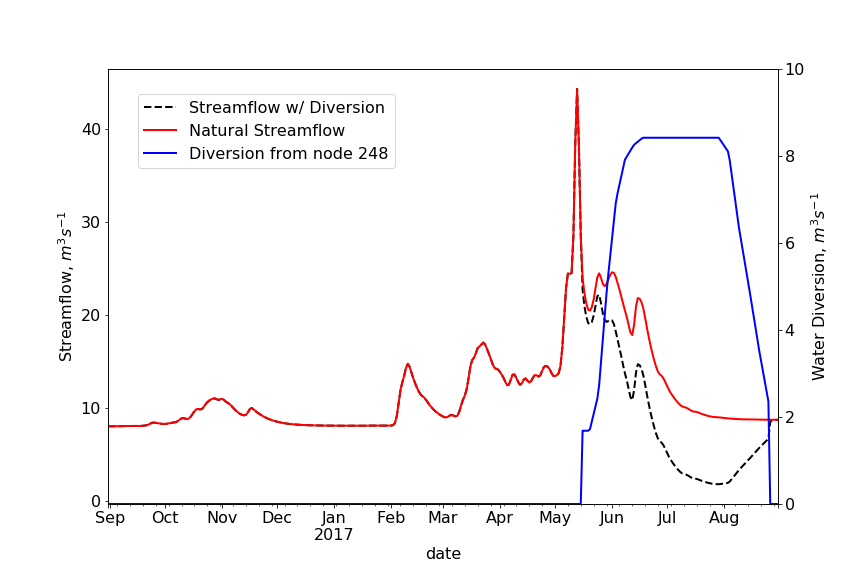
\includegraphics[width=\textwidth]{Figures/248_streamflow_diversion.png}
% \label{fig:ts_q_div}
% \caption{[WARNING: PLACEHOLDER FIGURE]Expected change in water allocation the 2012 drought as a percentage of the 2009 baseline allocation for three selected irrigated crops.}
% \end{figure}


 The extent of land allocated to irrigated crops is, of course, an indication of the agricultural water demands. In general, agricultural water use is higher in counties that are closer to the river headwaters. Counties in the headwaters of the Missouri river and upstream tributaries (Jefferson, Madison and Gallatin Rivers, see Figure \ref{fig:hydro_network}), in the southwestern quadrant of the state, as well as counties in the upper course of the Yellowstone river in south central Montana, have some of the highest agricultural water consumption in the state, putting a significant amount of strain on the water supplies. This agricultural water consumption pattern is clearly represented in the simulated total agricultural applications per county (Figure \ref{fig:total_water_map}). The model underestimated the total agricultural water use in all counties (negative relative errors), however the relative underestimations are in general modest. Large relative errors in the predictions often occur in counties with relatively low observed supplemental irrigation.    

\begin{figure}
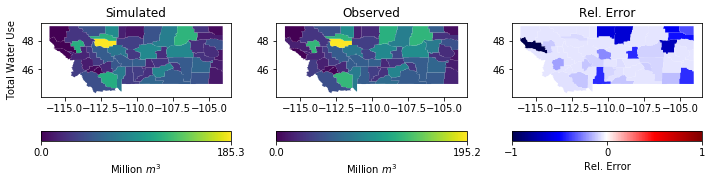
\includegraphics[width=0.9\textwidth]{Figures/total_water_use.pdf}
\label{fig:total_water_map}
\caption{Comparison between simulated (left panel) and observed (center panel) total agricultural water applications per county for year 2017. Right panel shows the relative prediction error defined as $\frac{simulated - observed}{observed}$. Counties with small amounts of observed irrigation can produce disproportionately large relative errors. For visualization purposes, the error scale has been clipped to values from -1 to 1. }
\end{figure}

Counties with high agricultural water use are expected to have the largest impacts on the hydrologic system. A strength of hydro-economic model is that it tracks the hydrologic impacts of agricultural activity. The spatial and temporal net effects of agricultural diversions on streamflows are shown in Figure \ref{fig:map_water_change}. Insets in Figure \ref{fig:map_water_change}a show simulated streamflows with and without the effects of water diversions for year 2017 in four nodes of the river network and the simulated water diversion rates from these nodes during the growing season. The standard profile of water diversion rates in all nodes followed the water demands associated with the progression of crops during the growing season. Water withdrawals start on the prescribed planting date of each crop, which for most crops is around May 15, increase as crops grow to full coverage, and finally taper down as crops mature before the prescribed harvesting date in late August. The impacts of water withdrawals on streamflows starts during the spring freshet, when streamflows are high, but it is typically maximal in late June or early August during low summer flows. When water diversions decline at the end of the summer, the model simulates the recovery of streamflows. 

\begin{figure}
\includegraphics[width=\textwidth]{Figures/FigureWaterUse.pdf}
\label{fig:map_water_change}
\caption{Simulated hydrologic conditions during the 2016-2017 water year. Insets in a) show  time series of simulated streamflows assuming no agriculture (red line), simulated streamflows with diversions (black dotted line), and agricultural water diversion (blue line) for four nodes in the river network. Panel b) shows the spatial impacts of agriculture on total annual streamflow volumes. $Delta$ Streamflow is the difference in total annual simulated streamflow volumes between the no agriculture reference model and the model with active agricultural diversions.}
\end{figure}

The spatially distributed nature of the hydrologic model naturally simulates the downstream impacts of agricultural activity. For instance, the inset associated with the easternmost node in Figure \ref{fig:map_water_change}a is not a diversion node, so there are no agricultural water withdrawals from this location, however water diverted upstream still reduces the natural flows in late spring and summer. To appreciate better the spatial extent of streamflow drawdowns, we produced a visualization of the total net impact of agriculture on the hydrologic network in 2017 (Figure \ref{fig:map_water_change}b). The net impact ($\Delta$ Streamflow) was produced by calculating the total annual water volume difference between natural flows and flows under agricultural withdrawals. Unsurprisingly, the most impacted river reaches are those that supply water to counties with high agricultural water applications, such as those in the headwaters of the Missouri river (c.f. Figure \ref{fig:total_water_map}), however the impact of water diversion often extends far downstream, affecting counties where agricultural water demands are low. 

\section{Discussion}

The implementation of the economic component of our hydro-economic model uses the stochastic and recursive data assimilation framework based on the ensemble Kalman filter proposed by Maneta and Howitt \citet{Maneta2014}, however the new implementation adopts the form of the optimality conditions for calibration proposed by \citet{Merel2011b} and \citet{Garnache2017}. The implementation of the positive mathematical programming methods proposed by these authors has two major advantages over the standard implementation used by \citet{Maneta2014}. One advantage is that it eliminates the need to solve an initial linear constrained optimization problem to identify the unknown Lagrange multipliers associated with land and water constraints \citep{Howitt1995}. Another important advantage is that it does not require a quadratic or exponential specification of the land cost function used in the standard implementation to provide the response function with the correct curvature \citep{Howitt1995, Howitt2012}.  

 Our analysis demonstrates that information on land use, crop evapotranspiration and crop production from existing and newer satellite-based remote sensing products contain sufficient information to calibrate the hydro-economic model presented here. It also shows that the recursive data assimilation methodology is effective for filtering out observation noise and identifying the correct model parameters within a relatively small number of assimilation cycles. Furthermore, The recursive updating nature of the filtering algorithm is ideal for model applications in non-stationary systems because it adapts the model calibration to the realities of the regional agriculture. Variations in the model parameters over time may be indicative of changes in the economic behavior of farmers triggered by external factors that may not be directly or easily detectable from satellite-based remote sensing information (e.g soil fertility) or due to shifting farmer perception or management practices. For instance, the recursive calibration for Beaverhead county (Figure \ref{fig:calibration2008-2015}), shows that parameter $\delta$, which represents the production returns to scale, is slowly increasing over time for irrigated alfalfa while remaining relatively stable for other crops. Values less than unity for this parameter indicate that crop production will increase exponentially less than a given increase in land and water allocated to this crop. Decreasing returns to scale reflect agricultural realities like the likelihood that crops expand to land of lessening quality, or the diminishing returns of additional water applications when crops are irrigated near their optimal level. Upward trends of this parameter signal technical or management improvements over our study period that increase productivity returns from land and water inputs. On the other hand, Parameter $mu$, which is a factor that represents the efficiency of the production system, seemed to decline for irrigated and non-irrigated spring wheat. Declines in this factor indicate loss of county production in these crops that cannot be explained by a reduction in the amount of land and water allocated to these crops. For instance, if may signal loss of soil fertility or declines in other inputs not explicitly included in the model. Note that the sensitivity of the model parameters to new observations is dependent on the value of $a$ in the parameter blending Eq. \eqref{eq:param_evolution}. This $a$ factor was prescribed at a value of 0.5 for this analysis, which provides a high level of smoothing and results in model parameter ensembles that represent long term conditions. Higher values of $a$ increase the calibration sensitivity to new observations, however at the expense of less stable parameter traces.
 
 An important characteristic of economic models of agricultural production calibrated using the PMP methodology is that there is no need to know with precision the production costs because the calibration algorithm approximates unknown or unspecified production costs by adjusting the $\lambda_{land,i}$ and $\lambda_{water,i}$. In our implementation of the optimality conditions, negative $\lambda_{i}$ values for land or water indicate that there are unobserved benefits associated with these inputs, which is to say that the observed production costs, $c_{land_i}$ and $c_{water,i}$, are overestimated. Conversely, a positive $\lambda_{i,l}$ value means that the observed production costs are under-estimated. In general, and in the case of Beaverhead county (Figure \ref{fig:calibration2008-2015}), irrigated crops typically have a negative value for $\lambda_{water,i}$, while positive values are more common in non-irrigated crops. 
 
 The capacity to estimate the value of $\lambda_{water,i}$ is an important characteristic of the calibration method, however this parameter is often the  most unstable during the data assimilation process and probably one of the largest sources of uncertainty in model predictions, as diagnosed by biases in component (2) of the innovation (Figure \ref{fig:innovation20082015}). Errors in the identification of this parameter may be the largest source of bias in the predictions of water and land allocation for years 2017 and 2018. 
 
 We found during our data assimilation experiments (not presented in this study) that the parameter ensembles are very sensitive to the uncertainty in some specific observations, especially observations of yield elasticity ($\overline{\pi}_W$) and supply elasticity ($\overline{\eta}$). If the noise to signal ratio in the observations was too high, the ensemble of model parameters converged to a biased solution even if the observation errors were unbiased, and this is one contributor to the prediction biases. \citet{Kanellopoulos2010} did similar forecast experiments using two variants of the positive mathematical programming method and reported model prediction sensitivities to the supply elasticity parameters and biases in model forecasts.  
 
 Our calibration methodology permits an unusual analysis of the model parameters and the quality of the model outputs. Commonly, hydro-economic models of agricultural production that are calibrated using any standard variation of the positive mathematical programming methodology are verified by reproducing the same baseline observations used for calibration. Model predictions under conditions different from those of the baseline are rarely verified with actual observations before the model is used in the simulation of design scenarios (\citep{Graveline2016}). This is because the empirical nature of the positive mathematical programming method limits the application of models calibrated using this methodology to conditions that are not too different from those of the calibration. Our results show that the model has forecasting skill even under the unusual flash drought conditions of 2017 and can correctly reproduce the spatial patterns of land and water allocation at county scales, albeit with some biases. Further research is necessary to understand the range of conditions under which the model still provides valid forecasts. 

 A major strength of our model is its ability to track the hydrologic impact of producer behavior. The hydrologic impacts of agricultural activity are maximal in early and mid August, right before crops mature and water diversions start to decline. This is also the period of lowest natural flows, therefore agricultural water diversions can exacerbate ecological stress in streams during years of low summer flows. However, the simulations also show that the temporal impacts of diversions are circumscribed to the irrigation season and streamflows recover quickly after diversions cease due to contributions from the substantial groundwater available in many of Montana's watersheds. The simulations also show that diversions also have an extensive spatial impact and their impact propagates downstream from counties where irrigation is most prevalent, such as these at the headwaters of the Missouri, Gallatin, and Yellowstone rivers. This pattern is correctly captured by the model. However, downstream impacts do not propagate unabated, and the recovery of streams is clearly visible in some reaches downstream of diversion nodes (Figure \ref{fig:map_water_change}. The recovery is caused by groundwater inflows into streams, which are known to be a key resilience mechanism for riverine ecosystems in the region. Groundwater is not yet extensively used as a source of water for irrigation in the region, and this may be the reason why the impacts of agricultural diversions are limited in space and in time. Conjunctive management of surface and groundwater may therefore be desirable to maintain the strength and resilience of Montana's rivers. 
 
 The results from the hydrologic component presented earlier are meant to illustrate the capabilities of the model, and should not be considered to be accurate. This model demonstration assumed 70\% efficiency in the water conveyance system and the irrigation technology for all counties. This efficiency parameter varies between counties and years and can have an important impact on the actual timing and volumes of diverted streamflows. Model refinements to improve the representation of these efficiencies are of major interest for state water managers and are underway. Another limitation of the current hydrologic component is that it does not yet include the effects of water impoundments. Artificial storage in dams and reservoirs and their release rules can have a large impact on the regional streamflow dynamics and provide additional resiliency by buffering and redistributing the spring freshet over a longer period. This model improvement is also a current priority.     

% Maybe talk some more about sensitivity and policy, like bottelneck regions and downstream disprotection if % rules do not limit upstream water use 
 

\section{Conclusions}

We describe the implementation of a hydro-economic model composed of a stochastic economic model of agricultural production and a rainfall-runoff and streamflow routing model that explicitly represents the spatial configuration of the regional water distribution network. The spatially-explicit nature of the hydrologic model permits to track the hydrologic impacts of producer activity. The economic component is designed to be continuously calibrated using remote sensing observations of land use, crop evapotranspiration and crop production. The calibration method is based on an implementationof the Positive Mathematical Programming methodology within a data assimilation framework that permits the recursive update of the model parameters when new remote sensing information becomes available.   The new formulation of the calibration methodology eliminates some of the limitations that have hindered the use of hydro-economic models to inform agricultural water management over large regions and temporal extents. Specifically, the model was designed to eliminate the need for expensive field surveys, reduce the problem of parameter overfitting to the conditions of the year and subset of farms used for calibration, and  reduce the false of precision that is associated with deterministic models.

The model is demonstrated for the state of Montana. We showed that satellite-based remote sensing retrievals of crop mix, land allocation, water allocation and crop yield, along with other ancillary information freely available online, contained sufficient information to correctly identify the parameters of the economic module. An interesting aspect of the recursive nature of the data assimilation methodology is that it permits to analyze the dynamics of the parameter ensembles over time, which may reveal trends in the biophysical and other factors that drive decision-making and are hard to observe directly, such as declines in land fertility, existence of hidden production costs, etc. The model was calibrated with eight years of observations (2008-2015) and effectively reproduced the observed levels of resource allocation of the 2008 baseline year used to spin-up the parameters. It also correctly predictive the spatial patterns of land and water allocation for years 2017 and 2018. Finally, we showed how the model can trace the effect of producer decision-making on the regional hydrologic system. This innovation of the model could be an important tool to understand how producer behavior affects the availability of water in the future, and how agricultural water use at county scales propagates through the hydrologic system to affect downstream users. The analysis of the time and propagation of streamflow drawdowns induced by agricultural water use may help identify regions that are at higher risk of water shortage during droughts.  

\section*{References}

\bibliography{manetaetal2020}

\appendix
\section{Hydrologic model}
\label{app:hydrologic_model}

The hydrologic system is simulated using a rainfall-runoff model coupled to a routing component that simulates streamflows in the regional stream network. We adapted the HBV model \citep{Bergstrom1995, Bergstrom1973} to simulate subcatchment-scale hydrologic processes (snowmelt, evapotranspiration, infiltration) and to transform precipitation into runoff and streamflow. Runoff that reaches the channel is routed through the stream network using the Muskingum-Cunge routing algorithm \cite{Chow1988}. In this appendix we provide here a description of the implementation of the algorithms.

\subsection{Rainfall Runoff component}

The HVB model \citep{Bergstrom1995, Bergstrom1973} is implemented as a mixture of gridded and vector-based operations to leverage the distributed nature of raster meteorological datasets while simultaneously taking advantage of the reduced computational burden of operating over polygons that aggregate runoff production over uniform hydrologic response units (HRUs). 

Snowpack accumulation and melt and soil processes are calculated over the uniform raster grid imposed by the meteorological inputs (precipitation, air temperature, and potential evapotranspiration). In the next two paragraphs subscript $i$ indicates that the variable or parameter is spatially distributed and is represented at grid point $i$. Superscript $t$ indicates that the variable is dynamic and its value is represented at time step $t$. Variables with no script or superscript indicate that the variable is spatially constant or time invariant. 

\paragraph{Precipitation and snowpack processes}      


Precipitation is partitioned between snowfall and rainfall using minimum and maximum daily air temperatures and a critical temperature threshold $Tc$ that determines the the snow-rain transition:

\begin{align}
Snow_i^t &= \left\{
	\begin{array}{ll}
	P_i^t &  Tmax_i^t < Tc_i \\   
	P_i^t * \frac{Tc_i - Tmin_i^t}{Tmax_i^t - Tmin_i^t} & Tmin_i^t < Tc_i < Tmax_i^t \\
	0 &  Tmin_i^t > Tc_i \\
	\end{array}
\right.\\
Rain_i^t &= P_i^t - Snow_i^t 	 
\end{align} 
\noindent where $P$ is precipitation (\si{\milli\metre\per\day}), $T_{max}$ and $T_{min}$ are maximum and minimum air temperature (\si{\degreeCelsius}), $Rain$ is liquid precipitation and $Snow$ is snowfall at pixel $i$ during time step $t$ (\si{\milli\metre\per\day}). Snowfall during day $t$ contributes to the snow water equivalent ($SWE$, (\si{\milli\metre})) of the snowpack:

\begin{equation}
SWE_i^t = SWE_i^{t-1} + Snow_i^t \Delta t
\end{equation}

The snowpack melt process is simulated using a degree day factor model occurs when average air temperature exceeds a air temperature threshold ($Tm$):

\begin{align}
Melt_i^t &= ddf_i * (Tav_i^t - Tm_i)  ]\text{ for } Tav_i^t > Tm_i \\
Rain_i^t &= P_i^t - Snow_i^t 	 
\end{align} 

\noindent where $Melt$ is the amount of water output from the snowpack (\si{\milli\metre\per\day}), $Tav$ is average air temperature over the time step (\si{\degreeCelsius}), and $ddf$ is the degree day factor (\si{\milli\metre\per\day\per\degreeCelsius}), an empirical parameter that represents the snowmelt rate per degree of air temperature above $Tm$. Any melt form the snowpack during time $t$ is subtracted from the snowpack storage ($SWE$) and added to the amount of water ponded in the surface: 

\begin{align}
Pond_i^t &= Pond_i^{t-1} + (Melt_i^t + Rain_i^t)\Delta t \\
SWE_i^t &= SWE_i^t - Melt_i^t \Delta t 	 
\end{align} 

\noindent where $Pond$ (\si{\milli\metre}) is liquid water available on the surface to infiltrate or produce runoff. 

\paragraph{Soil processes}  
Recharge into the soil system occurs when liquid water ponding the surface infiltrates into the soil. Ponded water that is not infiltrated increases the topsoil compartment that generates fast runoff. The fraction of ponded water that infiltrates into the soil is a exponential function of the relative water storage in the soil: 

\begin{align}
\Delta SM_i^t &= Pond_i^t * \left(1 - \frac{SM_i^t}{FC_i^t} \right)^\beta \\
\end{align} 

\noindent where $SM$ (\si{\milli\metre}) is the amount of water in the soil compartment, $FC$ (\si{\milli\metre}) is the maximum amount of water soil can hold before water starts percolating to the groundwater system, and $beta$ (dimensionless) is an empirical parameter. Simultaneously, actual evapotranspiration ($AET$, \si{\milli\metre\per\day}) reduces the amount of water storage in the soil and is also controlled by the degree of saturation of the soil (ration of $SM$ to $FC$). 

\begin{align}
AET_i^t &= PET_i^t * \left(\frac{SM_i^t}{FC_i * LP_i} \right)^l	 \\
\end{align} 

\noindent where $PET$ is potential evapotranspiration (\si{\milli\metre\per\day})) and $l$ is an empirical dimensionless parameter. Infiltration and actual evapotranspiration control the dynamics of water storage in the soil and amount of surface water that generates fast runoff:

\begin{align}
SM_i^t &= SM_i^{t} + \Delta SM_i^t - AET_i^t \Delta t\\
OVL_i^t &= Pond_i^t - \Delta SM_i^t
\end{align}

\noindent where $OVL$ (\si{\milli\metre}) is water that recharges the upper (near-surface) runoff-generating compartment.

\paragraph{Percolation and runoff generation}
Excess water in the topsoil and in two groundwater compartments generate outflow that represent fast and intermediate runoff and baseflow. These processes are implemented at the HRU level. For this, calculations about overland flow generation and soil moisture performed at the grid level are averaged over subwatersheds representing HRUs. Spatial arithmetic averaging soil water storage over all grid cells $i$ contained within a given HRU $j$ is represented using angle brackets $<.>$. The mass balance and percolation of water from the soil upper to the soil lower zone is implemented as:

\begin{align}
Rech_j^t &= <OVL_i^t>_j + <max(SM_i^t - FC_i, 0)>_j\\
SUZ_j^t &= SUZ_j^{t-1} + Rech_j^t + Pond_j^t - Q0_j^t\Delta t - Q1_j\Delta t - PERC_j\\
SLZ_j^t &= SLZ_j^{t-1} + PERC_j - Q2 \Delta t
\end{align}

\noindent $Rech$ (\si{\milli\meter}) is water storage in the near-surface compartment that generates fast runoff, $SUZ$ (\si{\milli\meter}) is the storage in the upper groundwater compartment, and $SLZ$ (\si{\milli\meter}) is water storage in the lower (deeper) groundwater compartment in HRU $j$ at time step $t$. $Q_0$, $Q_1$, and $Q_2$ (\si{\milli\meter\per\day}) are specific runoff rates from the soil surface, and the upper and lower soil zones:

\begin{align}
Q0_j^t &= max((SUZ_j - HL1_j) * \frac{1}{CK0_j}, 0.0)\\ 
Q1_j^t &= SUZ_j * \frac{1}{CK1_j}\\
Q2_j^t &= SLZ_j * \frac{1}{CK2_j}\\
Qall_j^t &= Q0_j^t + Q1_j^t + Q2_j^t
\end{align}

\noindent where $HL1$ (\si{\milli\meter}) is an empirical water storage threshold the triggers the generation of fast runoff, and $CK0$, $C10$, $CK2$ (\si{\day}) are empirical parameters representing the characteristic drainage time of each of the compartments. 
Total outflow from HRU $j$ on day $t$ is distributed over time to produce the catchment response by convoluting the output of HRU $j$ by triangular standard unit hydrograph with base $M_{base}$. 

\begin{align}
Q_j^t &= \sum_{i=1}^{M_{base}} Qall_j^{t-i+1} U(i) \\
U(i) &= \left\{
\begin{array}{ll}
\frac{4}{M_{base}^2}*i & 0 < i < M_{base}/2 \\
-\frac{4}{M_{base}^2}*i + \frac{4}{M_{base}} &  M_{base}/2 < i < M_{base} \\
\end{array}
\right.
\end{align}

\noindent where $U$ is a triangular hydrograph of area \num{1} and a base $MAXBAS$ (\si{\day})representing the hydrograph duration .  

\subsection{Routing component}

The response at the end of each $HRU$ is routed through the stream network using the Muskingum-Cunge routing model. In this model the storage in each stream reach $k$ is given by the following discharge-storage equation:

\begin{align}
S_k^t &= K\left[eQ_{in} + (1 - e)Q_{out} \right],
\end{align}

which has parameters $K$ (\si{\day}) and $e$ (dimensionless) controlling, respectively, the celerity and dispersion of the wave routed through the channel. 

Substituting this relationship in a finite-difference form of the continuity equation $\frac{S_j^{t+1} - S_j^{t}}{\Delta t} = Q_{in} - Q_{out}$ for a multi-reach system with lateral inflows injected upstream of reach draining $HRU$ $j$ at average constant rate through time step $t$ $q_{j}^{t+1}$ yields:

\begin{align}
&Q_j^{t+1}\left[K_j(1 - e_j) + 0.5\Delta t  \right] + Q_{j-1}^{t+1}\left[K_je_j - 0.5\Delta t  \right]  \\
&= Q_j^{t}\left[K_j(1 - e_j) - 0.5\Delta t  \right] + Q_{j-1}^{t}\left[K_je_j + 0.5\Delta t  \right]\\
&+ q_{j}^{t+1}\left[K_j(1 - e_j) + 0.5\Delta t  \right]
\end{align}

Each of the $HRUs$ contains one reach with an upstream and a downstream node. Streamflows for each of the $j=1,...,J$ reaches are integrated over time using a first-order explicit finite difference scheme. The system of $J$ equations can be assembled as a linear system of the form:    

\begin{align}\label{eq:linearsystem}
\mathbf{A}\mathbf{Q^{t+1}} = \mathbf{B} 
\end{align}

where $\mathbf{Q^{t+1}}$ is the vector of unknown streamflows at time $t+1$ for each of the $J$ reaches of the network that is solved each time step. Matrices $\mathbf{A}$ add $\mathbf{B}$ are functions of the model parameters and streamflows at timestep $t$:
\begin{align}
\mathbf{A}&\equiv (\mathbf{a} + \mathbf{\Phi} \mathbf{b})^T\\
\mathbf{B}&\equiv (\mathbf{d} + \mathbf{\Phi}\mathbf{c})^T\mathbf{Q}^t + \mathbf{I}(\mathbf{a\odot q}^{t+1})
\end{align}

where $\mathbf{\Phi}$ is a $JxJ$ sparse connectivity (0,1)-matrix where the elements indicate if two pairs of nodes are connected. Flow direction is from nodes in the rows to nodes in the columns. Rows representing the upstream node of $HRUs$ that drain an outlet node (exit the domain) are all zero. Finally,

%\begin{align}
%(\mathbf{a} + \mathbf{\Phi} \mathbf{b})\mathbf{Q^{t+1}} = (\mathbf{d} + %\mathbf{\Phi}\mathbf{c})\mathbf{Q^t} + \diag(\mathbf{a})*\mathbf{q^{t+1}}
%\end{align}

\begin{align}
\mathbf{a} &= \mathbf{I} (\mathbf{K}-\mathbf{K\odot e}) + dt * 0.5\\
\mathbf{b} &= \mathbf{I} (\mathbf{K\odot e}) - dt * 0.5\\
\mathbf{c} &= \mathbf{I} (\mathbf{K}-\mathbf{K\odot e}) - dt * 0.5)\\
\mathbf{d} &= \mathbf{I} (\mathbf{K\odot e}) + dt * 0.5
\end{align}

\noindent where $\mathbf{K}$ is the identity matrix of order $J$, $\mathbf{K}$ and $\mathbf{e}$ are column vectors holding parameters $K$ and $e$ for each of the $N$ reaches in the network. The $\odot$ operator denotes the Schur (elementwise) product between two vectors.
The solution of \eqref{eq:linearsystem} becomes unstable if $\Delta t > 2 * K_j * (1 - e_j)$. To ensure robust and stable solution an adaptive time stepping scheme was implemented. In this scheme, the default time step is reduced by an integer fraction until the the stability condition is satisfied in all reaches. 
%\appendix
\section{Economic model}
\label{app:economic_model}

Here we briefly outline the economic optimization program using the standard Positive Mathematical Programming (PMP), following \citet{Howitt1995, Merel2011b} and \citet{Garnache2017}. The economic program is implemented in two step: in the first step, parameters for the economic model are calibrated such that the program mimics the observed land and water use decisions. In the second step, the model simulates farmer's land use and water use responses given these model parameters along with other exogenous factors such as availability of supplemental irrigation water. The following subsections briefly outline the calibration and the simulation process at each simulation time. 

\subsection{Calibration}
\label{app:economic_model_calib}
The fundamental aspect of our economic program is that farmers allocate resources with the objective of maximizing net revenues, where the revenue function follows a generalized constant elasticity of substitution (CES) functional form: 
\begin{equation}\label{eq:econ_calibration}
    \begin{split}
    \max _ { x _ { land,i } , x _ { water,i } } & \quad \sum _ { i } \left\{ p _ { i } \mu _ { i } \left[ \beta _ { land,i } x _ { land,i } ^ { \rho _ { i } } + \beta _ { water,i } (x_{precip,i} + x _ { water,i }) ^ {\rho _ { i } } \right] ^ { \frac { \delta _ { i } } { \rho _ { i } } } \right.\\
    & \left. \quad - \left( c _ { land,i } + \lambda _ { land,i } \right) x _ { land,i } - \left( c _ { water,i } + \lambda _ { water,i } \right) x _ { water,i } \vphantom{\sum_i} \right\} \\
    \text{subject to} & \quad \sum _ { i } x _ { land,i } \leq \overline { L } \left[ \overline { \lambda } _ { land } \right] \\ 
    & \quad \sum _ { i } x _ { water,i } \leq \overline { W } \left[ \overline { \lambda } _ { water } \right] \\
    & \quad x_{land,i}, x_{water,i} \geq 0 \\
    \end{split}
\end{equation}
where $i = 1,...,I$ indexes crops; $l=land,water$ indexes land and water inputs. We differentiate water inputs into an exogenous component $x_{precip,i}$, which captures water provided by natural sources like precipitation, and an endogenous component $x_{water,i}$, which captures supplemental irrigation water provision. Total water application will be the summation of the two, i.e.
\begin{equation*}
    x^*_{water,i} \equiv x_{precip,i} + x_{water,i}
\end{equation*}

The unknown parameters in Equation~\ref{eq:econ_calibration} are $\mu _ { i } , \beta _ { i l } , \rho _ { i } , \delta _ { i } , \lambda _ { i l } , \overline { \lambda } _ { 1 }$; and the known values are:

\begin{itemize*}
    \item $\overline { \eta } _ { i }$: exogenous supply elasticity for crop i (\% change in supply over \% change in crop price)
    \item $\overline { q } _ { i }$: observed crop production for crop $i$
    \item $\overline { x } _ { land,i }$: observed land allocation for crop $i$
    \item $\overline { x } _ { water,i} ^{*}$: observed ET (total) for crop $i$
    \item $\overline { y } _ { i W}$: reference yield elasticity with respect to water for crop $i$ (\% change in production over \% change in total ET)
    \item $\sigma_i$: elasticity of substitution for crop $i$
    \item $p_i$: unit price of crop $i$
    \item $c_{il}$: per-unit input costs of production for crop $i$, input $l$
    \item $\overline { L }$: total arable land
    \item $\overline{W}$: total amount of supplemental irrigation water available
\end{itemize*}

Given the above maximization problem, the unknown parameters can be calibrated via positive mathematical programming, using the following set of calibration equations: 

\begin{equation}\label{eq:optimality_program}
    \begin{split}
        & \rho _ { i } = \frac { \sigma _ { i } - 1 } { \sigma _ { i } } \text { for } i = 1 , \ldots , I \\
        & \overline { \eta } _ { i } = \frac { \delta _ { i } } { 1 - \delta _ { i } } \left\{ 1 - \frac { \frac { b _ { i } } { \delta _ { i } \left( 1 - \delta _ { i } \right) } } { \sum _ { j } \left[ \frac { b _ { j } } { \delta _ { j } \left( 1 - \delta _ { j } \right) } + \frac { \sigma _ { j } b _ { j } \overline { y } _ { j W } } { \delta _ { j } \left( \delta _ { j } - \overline { y } _ { j W } \right) } \right] } \right\} \text { for } i = 1 , \ldots , I , \text {where } b _ { i } = \frac { \overline { x } _ { land,i } ^ { 2 } } { p _ { i } \overline { q } _ { i } } \\
        & \overline {y}_{iW} = \delta _ { i } \left( \frac { \beta _ { water,i } \overline { x } _ { water,i } ^ { * \rho _ { i } } } { \beta _ { land,i } \overline { x } _ { land,i } ^ { \rho _ { i } } + \beta _ { water,i } \overline { x } _ { water,i } ^ { * } \rho _ { i } } \right) \text { for } i = 1 , \ldots , I \\
        & \beta _ {land, i  } + \beta_{water,i} = 1 \text { for } i= 1 , \ldots , I \\
        & \overline { q } _ { i } = \mu _ { i } \left[ \beta _ { land,i } \overline { x } _ { land,i } ^ { \rho _ { i } } + \beta _ { water,i } \overline { x } _ { water,i } ^ { * \rho _ { i } } \right] ^ { \frac { \delta _ { i } } { \rho _ { i } } } \text { for } i = 1 , \ldots , I \\
        & \overline { \lambda } _ { 1 } = \frac { \sum _ { i } \left[ p _ { i } \overline { q } _ { i } \left( \delta _ { i } - \overline { y } _ { i W } \right) - c _ { land,i } \overline { x } _ { land,i } \right] \overline { x } _ { land,i } } { \sum _ { i } \left( \overline { x } _ { land,i } ^ { 2 } \right) } \\
        & p _ { i } \overline { q } _ { i } \left( \delta _ { i } - \overline { y } _ { i W } \right) = \left( c _ { land,i } + \lambda _ { land,i } + \overline { \lambda } _ { 1 } \right) \overline { x } _ { land,i } \text { for } i = 1 , \ldots , I \\
        & p _ { i } \overline { q } _ { i } \overline { y } _ { i W } = \left( c _ { water,i } + \lambda _ { water,i } \right) \overline { x } _ { water,i } ^ { * } \text { for } i = 1 , \ldots , I
    \end{split}
\end{equation}

\subsection{Simulation}
After calibrating the model parameters, the optimization framework can now be used to analyze how farmer behaviors will change given changes in exogenous environmental and economic factors, including water availability, crop prices, and production costs. 

The simulation problem is given by the following maximization problem:
\begin{equation}\label{eq:econ_simulation}
\begin{split}
    \max _ { x _ { land,i } , x _ { water,i }} &  \sum _ { i } \left\{ p _ { i } \mu _ { i } \left[ \beta _ { land,i } x _ { land,i } ^ { \rho _ { i } } + \beta _ { water,i } x _ { water,i } ^ { * } \rho _ { i } \right] ^ { \frac { \delta _ { i } } { \rho _ { i } } } \right.\\
    & \left. - \left( c _ { land,i } + \lambda _ { land,i } \right) x _ { land,i } - \left( c _ { water,i } + \lambda _ { water,i } \right) x _ { water,i } \vphantom{\sum_i} \right\} \\
    \text{subject to } & \sum _ { i } x _ { land,i } \leq \overline { L } \left[ \overline{\lambda} _ { land } \right] \\
    & \sum _ { i } x _ { water,i } ^ { * } \leq \overline { W } \left[ \overline{\lambda} _ { water } \right] \\
    & \text {and } x _ { water,i } \geq 0 \left[ \xi _ { i } \right]
\end{split}
\end{equation}
where the unknown values are $x _ { land,i } , x _ { water,i }$, the land and water inputs for crop $i$; $q _ { i }$, the total production for crop $i$; and $\overline{\lambda} _ { land }, \overline{\lambda} _ { water }, \xi$, the Lagrangian multipliers. The known values include:
\begin{itemize*}
    \item $\mu _ { i } , \beta _ { i l } , \rho _ { i } , \delta _ { i } , \lambda _ { i l }$: model parameters determined from the calibration equations
    \item $p _ { i } , c _ { i l } , x_{precip,i}, \overline { L } , \overline { W }$: crop prices, per unit production costs, water from natural sources, total arable land, and total supplemental irrigation water (same as in the calibration equation~\ref{eq:econ_calibration}).
\end{itemize*}

The simulation equations to solve the above maximization problem are given by:
\begin{equation}
\begin{split}
    & \frac { p _ { i } \delta _ { i } q _ { i } \beta _ { land,i } x _ { land,i } ^ { \rho _ { i } } } { \beta _ { land,i } x _ { land,i } \rho _ { i } + \beta _ { water,i } x _ { water,i } ^ { * \rho _ { i } } } = \left( c _ { land,i } + \lambda _ { land,i } + \lambda _ { 1 } \right) x _ { land,i } \text { for } i = 1 , \ldots , I \\
    & \frac { p _ { i } \delta _ { i } q _ { i } \beta _ { water,i } x _ { water,i } ^ { * \rho _ { i } } } { \beta _ { land,i } x _ { land,i } ^ { \rho _ { i } } + \beta _ { water,i } x _ { water,i } ^ { * } \rho _ { i } } = \left( c _ { water,i } + \lambda _ { water,i } + \lambda _ { 2 } + \xi _ { i } \right) x _ { water,i } ^ { * } \text { for } i = 1 , \ldots , I \\
    & q _ { i } = \mu _ { i } \left[ \beta _ { land,i } x _ { land,i } ^ { \rho _ { i } } + \beta _ { water,i } x _ { water,i } ^ { * \rho _ { i } } \right] ^ { \frac { \delta _ { i } } { \rho _ { i } } } \text { for } i = 1 , \ldots , I \\
    & \sum _ { i } x _ { land,i } = \overline { L } \text { for } i = 1 , \ldots , I \\
    & \sum _ { i } x _ { water,i } ^ { * } = \overline { W } \text { for } i = 1 , \ldots , I
\end{split}
\end{equation}

The simulation model will be able to recover farmers land and water use choices, $x_{land,i}$ and $x_{water,i}$, under the new set of exogenous conditions. The model will also be able to recover shadow values with respect to land and water inputs, $\overline{\lambda} _ { land }$ and $\overline{\lambda} _ { water }$.

Note that this system of equations requires that the water constraint is binding. If the water constraint is non-binding, complementary slackness conditions need to be built to allow for the case in which $\lambda _ { water } = 0$.




\end{document}


